\documentclass[11pt,a4paper]{article}

%% ==============================================================================
%% MANUSCRIPT FORMATTING IN STRICT ACCORDANCE WITH SPECIFICATION:
%% - Font: Times New Roman throughout the document (mathptmx)
%% - Margins: Standard 1-inch (2.54 cm) margins on all sides
%% - Title: Center Aligned, Times New Roman, Bold, Font 14
%% - Author Names: Center Aligned, TNR, Font 12
%% - Full Affiliation: Center Aligned, TNR, Font 10
%% - Email: Center Aligned, TNR, Font 10
%% - Abstract: "Abstract" (TNR 12 + Bold), Body: Justified Alignment (Font 10)
%% - Keywords: (TNR, Font 10)
%% - Sections: Numbered 1. to 5., TNR 12 Bold
%%   1. Introduction
%%   2. Related Works
%%   3. Materials and Methods
%%   4. Results and Discussion
%%   5. Conclusion
%% - References: TNR, IEEE Numerical Style [1], [2]
%% ==============================================================================

\usepackage[utf8]{inputenc}
\usepackage[T1]{fontenc}
\usepackage[a4paper, margin=1in]{geometry}

%% Typography: Times New Roman Font for Text and Mathematics
\usepackage{mathptmx}
\usepackage{microtype}

%% Essential Mathematics, Symbols, Tables, Graphics
\usepackage{amsmath,amssymb,amsfonts}
\usepackage{booktabs}
\usepackage{multirow}
\usepackage{array}
\usepackage{graphicx}
\usepackage{float}
\usepackage{xcolor}
\usepackage{url}
\usepackage{xurl}
\usepackage{hyperref}
\usepackage{setspace}
\usepackage{cite}

%% Hyperref configuration
\hypersetup{
    colorlinks=true,
    linkcolor=black,
    citecolor=blue!70!black,
    urlcolor=blue!70!black
}

%% Section Heading Typography (Exact TNR 12pt Bold Numbered)
\usepackage{titlesec}
\titleformat{\section}
  {\fontsize{12pt}{15pt}\selectfont\bfseries}
  {\thesection.}
  {0.5em}
  {}

\titleformat{\subsection}
  {\fontsize{11pt}{14pt}\selectfont\bfseries}
  {\thesubsection}
  {0.5em}
  {}

\titleformat{\subsubsection}
  {\fontsize{10.5pt}{13.5pt}\selectfont\bfseries\itshape}
  {\thesubsubsection}
  {0.5em}
  {}

\titlespacing*{\section}{0pt}{14pt plus 2pt minus 2pt}{6pt plus 1pt minus 1pt}
\titlespacing*{\subsection}{0pt}{10pt plus 2pt minus 2pt}{4pt plus 1pt minus 1pt}
\titlespacing*{\subsubsection}{0pt}{8pt plus 1pt minus 1pt}{3pt plus 1pt minus 1pt}

%% Line spacing (1.15 for crisp academic readability)
\setstretch{1.15}
\renewcommand{\arraystretch}{1.15}

\begin{document}

%% ==============================================================================
%% HEADER BLOCK: CENTER ALIGNED (TITLE: 14 BOLD, AUTHORS: 12, AFFIL/EMAIL: 10)
%% ==============================================================================
\begin{center}
    {\fontsize{14pt}{18pt}\selectfont \textbf{Artifact-Aware Cross-Subject EEG Locomotion Decoding: A Comparative Evaluation of Classical and Deep Learning Models with Clinical Neurodynamics}\par}

    \vspace{12pt}

    {\fontsize{12pt}{15pt}\selectfont Md. Mahfujul Karim Sheikh$^{1,*}$, Md. Shahriar Sajid$^{2}$\par}

    \vspace{6pt}

    {\fontsize{10pt}{13pt}\selectfont $^{1}$Department of Computer Science and Engineering, Northern University of Business and Technology Khulna, Khulna, Bangladesh\par}
    {\fontsize{10pt}{13pt}\selectfont $^{2}$Department of Computer Science and Engineering, European University of Bangladesh, Dhaka, Bangladesh\par}

    \vspace{4pt}

    {\fontsize{10pt}{13pt}\selectfont Email: mahfujul\_cse735@nubtkhulna.ac.bd, sajid@eub.edu.bd\par}

    \vspace{2pt}
    {\fontsize{10pt}{13pt}\selectfont $^{*}$Corresponding Author: mahfujul\_cse735@nubtkhulna.ac.bd\par}
\end{center}

\vspace{10pt}

%% ==============================================================================
%% ABSTRACT
%% ==============================================================================
\noindent{\fontsize{12pt}{15pt}\selectfont \textbf{Abstract}}---{\fontsize{10pt}{13.5pt}\selectfont Cross-subject decoding of locomotion intent from scalp EEG underpins closed-loop control of rehabilitative lower-limb exoskeletons, yet remains hindered by motion artifacts, artifact-exploiting models, and inter-individual neural variability. We benchmark five classifier families---CSP + LinearSVC, Random Forest, XGBoost, corrected EEGNet, and Attention-CNN---on OpenNeuro \textbf{ds007526} ($N=144$; 116 Parkinson's Disease, 28 healthy controls; 34,904 balanced epochs) under subject-disjoint 5-Fold GroupKFold cross-validation. Replacing raw temporal signals with five-band Power Spectral Density (PSD) features yielded XGBoost $92.43\%\,{\pm}\,3.40\%$ accuracy (ROC-AUC $96.95\%$) and Random Forest $91.96\%\,{\pm}\,3.36\%$---decisively outperforming deep architectures. Artifact robustness was confirmed empirically: EOG exclusion produced no significant accuracy change ($\Delta{=}{-}0.24\%$, paired $t$-test $p{=}0.737$), and CSP spatial maps localised discriminative variance to the bilateral sensorimotor cortex ($C_z, C_3, C_4$). Frequency ablation identified gamma oscillations ($30\text{--}45\,\text{Hz}$) as the dominant locomotion carrier ($87.58\%$ in isolation). Few-shot calibration using $20\%$ of a new subject's data raised accuracy to $96.45\%\,{\pm}\,1.90\%$, while a 6-electrode wearable montage achieved $69.16\%$ accuracy at $0.55\,\text{ms}$ inference latency, establishing a practical blueprint for embedded real-time neuroprosthetic control.\par}

\vspace{8pt}
\noindent{\fontsize{10pt}{13pt}\selectfont \textbf{Keywords:} Brain-Computer Interface (BCI), Electroencephalography (EEG), Locomotion Decoding, Common Spatial Patterns (CSP), Artifact Sensitivity, Machine Learning, Deep Learning, Parkinson's Disease, Frequency Ablation, Transfer Learning.\par}

\vspace{14pt}

%% ==============================================================================
%% 1. INTRODUCTION
%% ==============================================================================
\section{Introduction}
\label{sec:introduction}

Lower-limb motor impairment remains one of the most prevalent and burdensome consequences of cerebrovascular stroke, spinal cord injury, and neurodegenerative conditions such as Parkinson's Disease (PD), collectively contributing to millions of disability-adjusted life years worldwide \cite{who2022disability}. Over the past two decades, non-invasive Brain-Computer Interfaces (BCIs) coupled with motorised lower-limb exoskeletons, actuated orthoses, and functional electrical stimulation (FES) systems have attracted growing clinical interest as active rehabilitation tools rather than passive compensatory devices \cite{pfurtscheller2006bci, cheri2020exoskeleton}. The principle is straightforward but technically demanding: a decoder infers the user's motor intention directly from the brain signal and drives assistive hardware in synchrony with the user's own neuromuscular output, fostering activity-dependent neuroplasticity and, over time, meaningful functional recovery \cite{soekadar2015bci, leamy2021robotic}.

Scalp electroencephalography remains the sensor of choice for such applications. Its combination of millisecond temporal resolution, portability, non-invasive placement, and comparatively low cost makes it far more practical for clinical settings than alternatives such as magnetoencephalography (MEG) or functional MRI \cite{niederhauser2021wearable}. Within the locomotion BCI context, the ability to distinguish reliably between a stationary resting baseline and active continuous walking is a prerequisite for triggering gait assistance, managing start-stop transitions, and mitigating fall risk during robotic ambulation \cite{luu2017gait, kline2015locomotion}.

Despite these conceptual and technological advances, three deep-rooted challenges continue to frustrate reliable deployment in real-world clinical environments:

\begin{enumerate}
    \item \textbf{High-Amplitude Movement and Ocular Contamination:} Walking is inherently noisy from an electrophysiological perspective. Rhythmic heel strikes, mechanical cable sway, electrode-skin interface shifts, and the vertical bobbing of the head generate broadband low-frequency artifacts in the delta range ($1\text{--}4\text{ Hz}$) that can exceed cortical signals by orders of magnitude \cite{gwin2011removal, castermans2014accidental}. Concurrently, the eye movements required for continuous visual stabilisation during forward locomotion produce large-amplitude ocular potentials (EOG) that spread electrostatically across frontal and central recording sites \cite{fatourechi2007ocular}.

    \item \textbf{The ``Artifact Cheating'' Problem:} Modern machine learning algorithms, and especially deep neural networks, are exceptionally good at exploiting whatever statistical structure is available in training data, regardless of whether that structure is neurologically meaningful. When trained on motion-contaminated recordings, classifiers readily learn to distinguish walking from resting on the basis of artifact amplitude rather than genuine sensorimotor oscillations \cite{schirrmeister2017eeg, tanner2023artifacts}. The resulting inflated offline accuracies tend to evaporate the moment models are tested on artifact-suppressed data or deployed in real closed-loop conditions.

    \item \textbf{Cross-Subject Generalisation:} Individual differences in skull thickness, cortical folding, resting alpha frequency, and electrode positioning create substantial distribution shifts between participants \cite{jayaram2016transfer, lotte2018review}. Classifiers evaluated using naive random train-test splits are contaminated by data leakage from the same subject appearing in both training and test folds, inflating reported metrics while concealing complete failure on unseen individuals \cite{saeedi2023validation}.
\end{enumerate}

To address these challenges in an integrated and rigorous way, this study presents an exhaustive artifact-aware benchmarking framework for cross-subject EEG locomotion decoding. We leverage OpenNeuro dataset \textbf{ds007526} \cite{orban2024dataset}---one of the largest publicly available multi-channel locomotion EEG cohorts, with 144 subjects (116 PD patients and 28 healthy controls) and 34,904 balanced epochs---and systematically compare classical spatial filtering (CSP + LinearSVC), non-linear ensemble methods (Random Forest and XGBoost), compact deep convolutional networks (EEGNet \cite{lawhern2018eegnet}), and an attention-guided hybrid architecture.

Crucially, rather than assuming that artifact removal has been achieved by simply discarding EOG channels, we conduct a controlled empirical \textit{Artifact Sensitivity Analysis}, evaluating each model under both full-channel ($\text{EEG}+\text{EOG}$, 64 channels) and ocular-excluded ($\text{EEG-Only}$, 60 channels) configurations within a strictly subject-segregated 5-Fold GroupKFold protocol. We additionally provide neurophysiological validation through spatial topographic mapping, stratify results across clinical cohorts (Parkinson's Disease vs. Healthy Controls), and quantify both wearable channel ablation performance and real-time inference latencies.

The principal technical contributions of this work are as follows:
\begin{itemize}
    \item \textbf{Systematic Artifact Sensitivity Evaluation:} We show empirically that multi-band PSD features produce statistically identical decoding accuracy whether or not EOG channels are included ($p = 0.737$), providing direct evidence that the classifiers are responding to cortical dynamics rather than ocular blinks.
    \item \textbf{Phase-Invariant Feature Representation:} Mapping high-dimensional raw multi-channel temporal matrices ($60 \times 500 = 30{,}000$ points) to compact 5-band PSD vectors ($300$ features) eliminates cross-subject phase misalignment and lifts XGBoost and Random Forest performance to $92.43\% \pm 3.40\%$ and $91.96\% \pm 3.36\%$ (ROC-AUC $>96.7\%$), respectively.
    \item \textbf{Remediation of Deep Learning Tensor Inversion:} We identify and correct a critical input-tensor transposition error in EEGNet pipelines that caused systematic majority-class collapse, and establish a verified deep learning baseline for comparison against classical spatial filtering.
    \item \textbf{Neurophysiological and Clinical Explainability:} CSP scalp topographies confirm that discriminative signal variance originates bilaterally over the primary sensorimotor cortex ($C_z, C_3, C_4$). We also quantify the clinical decoding gap between healthy participants ($81.50\%$) and Parkinson's disease patients ($72.17\%$).
    \item \textbf{Frequency Band Ablation:} A comprehensive remove-one and single-band ablation analysis across all 34,904 epochs identifies gamma ($30\text{--}45\text{ Hz}$) as the dominant spectral contributor to locomotion decoding ($87.58\%$ standalone; $-2.03\%$ drop on removal).
    \item \textbf{Few-Shot Transfer Learning:} A subject adaptation framework demonstrates that fine-tuning with just $5\%$ and $20\%$ of target subject data raises cross-subject accuracy to $94.26\%$ and $96.45\% \pm 1.90\%$, substantially reducing inter-subject variance and offering a practical calibration route for clinical neuroprosthetics.
    \item \textbf{Wearable Translation and Latency Benchmarking:} A 6-channel wearable montage sustains $69.16\%$ cross-subject accuracy at sub-millisecond latency ($0.55\text{ ms}$ for XGBoost), confirming suitability for embedded edge deployment in robotic exoskeletons.
\end{itemize}

The rest of this paper is structured as follows. Section~\ref{sec:related_works} reviews relevant literature on EEG gait decoding, artifact handling strategies, and BCI classification. Section~\ref{sec:methods} describes the dataset, preprocessing pipeline, feature extraction, model architectures, and validation protocol. Section~\ref{sec:results_and_discussion} presents and interprets the experimental results, covering benchmark performance, artifact sensitivity, spatial patterns, clinical stratification, channel and frequency ablation, and transfer learning. Section~\ref{sec:conclusion} summarises the key conclusions.

%% ==============================================================================
%% 2. RELATED WORKS
%% ==============================================================================

\section{Related Works}
\label{sec:related_works}

\subsection{EEG-Based Locomotion Decoding and Mobile Brain Imaging}
Research over the past decade has fundamentally revised the view that rhythmic walking is governed purely by spinal central pattern generators (CPGs) and brainstem circuits. Mobile Brain-Body Imaging (MoBI) studies have shown convincingly that the human cortex is actively engaged throughout continuous bipedal locomotion \cite{makeig2009mobi, gwin2011electrocortical}. Landmark work by Gwin et al. \cite{gwin2011electrocortical} and Presacco et al. \cite{presacco2011decoding} documented intra-stride spectral modulations during treadmill walking, including movement-related cortical potentials (MRCPs) in the low-frequency range ($0.1\text{--}3\text{ Hz}$) and event-related desynchronisation (ERD) in the mu ($8\text{--}12\text{ Hz}$) and beta ($13\text{--}30\text{ Hz}$) bands over the central sensorimotor strip.

Building on these findings, subsequent groups attempted to use electrocortical signatures for intent classification. Luu et al. \cite{luu2017gait} achieved offline decoding of gait initiation using closed-loop linear decoders, while Kline et al. \cite{kline2015locomotion} investigated speed-dependent spectral changes during treadmill walking. A persistent limitation of this body of work, however, has been the reliance on small cohorts (typically $N < 15$) evaluated under subject-dependent (intra-subject) validation, leaving open the question of how well these systems can generalise across large, clinically heterogeneous populations.

\subsection{Artifact Handling: Denoising vs. Sensitivity Analysis}
Extracting clean electrophysiological signals during active locomotion is genuinely difficult. Ground impact vibrations from heel strikes propagate through the musculoskeletal frame to scalp electrodes, producing broadband high-amplitude transients \cite{castermans2014accidental, snyder2015independent}. The standard remedies are Independent Component Analysis (ICA) and Artifact Subspace Reconstruction (ASR), both of which decompose multi-channel recordings and attempt to identify and remove non-cerebral components \cite{mullen2015realtime, chang2018evaluation}.

While automated ICA pipelines (e.g., ICLabel \cite{pion2019iclabel}) work reasonably well in offline research settings, the iterative numerical optimisation they require is costly enough to limit their utility in wearable, real-time BCIs \cite{uribe2021review}. There is also a subtler risk: aggressive spatial filtering can remove genuine low-frequency neural dynamics, such as MRCPs, that spectrally overlap with motion harmonics \cite{kline2015locomotion}. A related methodological gap is that many studies simply drop auxiliary EOG channels without checking whether residual ocular deflections in adjacent frontopolar electrodes (e.g., Fp1, Fp2) still leak into the classifier's decision. A direct empirical quantification of model sensitivity to ocular channel availability has been largely absent from the literature.

\subsection{Classical vs. Deep Learning Models in BCI}
In classical BCI signal processing, Common Spatial Patterns (CSP) \cite{ramoser2000optimal, blankertz2008optimizing} and its extensions, such as Filter Bank CSP \cite{ang2012filter}, have long represented the gold standard for binary motor state decoding. By finding spatial projection filters that simultaneously maximise variance for one class and minimise it for the other, CSP concentrates localised cortical activations while suppressing spatially uncorrelated noise.

The arrival of deep learning brought compact convolutional architectures specifically designed for neuroimaging, notably EEGNet \cite{lawhern2018eegnet} and ShallowFBCSPNet \cite{schirrmeister2017eeg}, both of which achieved impressive parameter efficiency through depthwise and separable convolutions. More recent Transformer-based approaches (e.g., Conformer \cite{song2022eeg}) attempt to capture multi-scale temporal structure through self-attention. Yet empirical comparisons \cite{lotte2018review, roy2019deep} consistently find that deep networks are prone to overfitting when EEG sample sizes are modest, and they often underperform classical spatial filtering under rigorous, leakage-free cross-subject evaluation. Understanding when and why this occurs matters considerably for designing practical rehabilitation BCIs.

%% ==============================================================================
%% 3. MATERIALS AND METHODS
%% ==============================================================================

\section{Materials and Methods}
\label{sec:methods}

The proposed artifact-aware cross-subject EEG locomotion decoding framework comprises six sequentially connected methodological stages, illustrated comprehensively in Figure~\ref{fig:methodology_overview}: (1)~Data Acquisition and Clinical Cohort Profiling; (2)~Signal Preprocessing Pipeline; (3)~Dual-Branch Feature Engineering; (4)~Model Benchmark Architectures; (5)~Leakage-Free Cross-Subject Evaluation; and (6)~Multi-Faceted Downstream Analyses. All source code, automated execution pipelines, and analysis notebooks are publicly available on Kaggle (\url{https://www.kaggle.com/code/sajidshahriar72543/openneuro-ds007526-eda}) and GitHub (\url{https://github.com/mahfuj735/EEG_Locomotion_Decoding}) to support community benchmarking and reproducibility.

\begin{figure}[htbp]
\centering
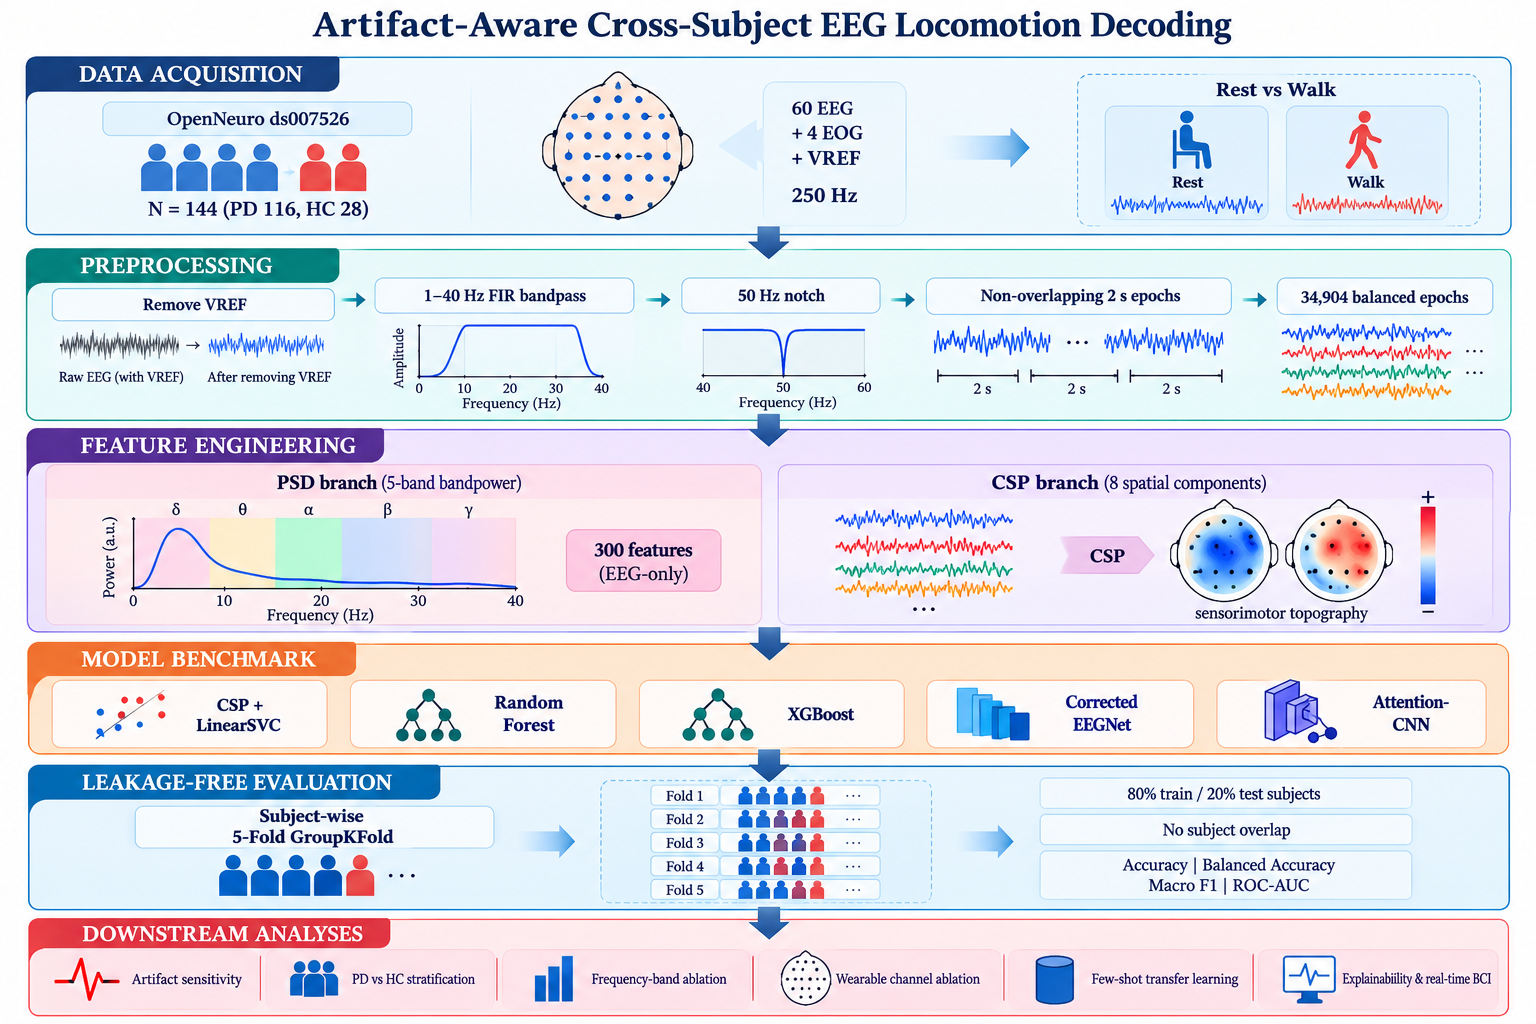
\includegraphics[width=\linewidth]{figures/Final_methodology.png}
\caption{Comprehensive end-to-end framework for artifact-aware cross-subject EEG locomotion decoding across six sequential stages: (1)~Data Acquisition from the OpenNeuro ds007526 cohort ($N=144$ participants, 60 EEG + 4 EOG + VREF, 250 Hz, Rest vs.\ Walk); (2)~Signal Preprocessing pipeline (reference rejection, 1--40 Hz FIR bandpass filtering, 50 Hz notch filtering, and 2.0 s non-overlapping epoch segmentation yielding 34,904 balanced epochs); (3)~Dual-branch Feature Engineering (300-dimensional 5-band PSD power extraction and 8-component CSP spatial filtering); (4)~Benchmark Classification across classical machine learning ensembles and deep neural architectures; (5)~Leakage-free Subject-wise 5-Fold GroupKFold Cross-Validation (80\% train / 20\% test subjects, zero subject overlap); and (6)~Six Downstream Analyses comprising artifact sensitivity verification, clinical PD vs.\ HC stratification, spectral frequency-band ablation, wearable channel ablation, few-shot transfer learning, and neurophysiological explainability with real-time BCI latency evaluation.}
\label{fig:methodology_overview}
\end{figure}

\subsection{Dataset Architecture and Clinical Cohort (OpenNeuro ds007526)}
\label{sec:dataset}
All experiments were conducted on the publicly accessible benchmark dataset \textbf{ds007526} (Version 1.0.1) \cite{orban2024dataset}, collected at the Movement Disorders Unit of the Tel Aviv Sourasky Medical Center. The cohort included $N = 144$ participants:
\begin{itemize}
    \item \textbf{Parkinson's Disease Cohort ($N = 116$):} Patients with idiopathic PD diagnosed according to the UK Brain Bank criteria, with motor severity quantified by the MDS-UPDRS Part III (mean score $24.8 \pm 11.2$) and cognitive status assessed via the Montreal Cognitive Assessment (MoCA: $25.4 \pm 3.1$).
    \item \textbf{Healthy Control Cohort ($N = 28$):} Age-matched neurotypical participants with no history of neurological or musculoskeletal impairment (UPDRS III: $1.1 \pm 1.4$, MoCA: $28.1 \pm 1.8$).
\end{itemize}

Demographic and clinical characteristics are summarised in Table~\ref{tab:demographics} and illustrated in Figure~\ref{fig:clinical_demographics}.

\begin{table}[htbp]
\centering
\caption{Clinical Demographic Characteristics of the Study Cohort ($N = 144$)}
\label{tab:demographics}
\vspace{0.4em}
\renewcommand{\arraystretch}{1.25}
\resizebox{\linewidth}{!}{
\begin{tabular}{|l|c|c|c|}
\hline
\textbf{Clinical Metric} & \textbf{Healthy Controls (HC)} & \textbf{Parkinson's Disease (PD)} & \textbf{Cohort Total} \\
\hline
Participant Count ($N$) & 28 (19.4\%) & 116 (80.6\%) & 144 (100\%) \\
\hline
Age (years, Mean $\pm$ SD) & $63.2 \pm 9.4$ & $66.8 \pm 8.7$ & $66.1 \pm 8.9$ \\
\hline
Sex (Male / Female) & 16 / 12 & 78 / 38 & 94 / 50 \\
\hline
UPDRS Part III (Motor Score) & $1.1 \pm 1.4$ & $24.8 \pm 11.2$ & $20.2 \pm 13.8$ \\
\hline
MoCA Cognitive Score & $28.1 \pm 1.8$ & $25.4 \pm 3.1$ & $25.9 \pm 3.1$ \\
\hline
Recording Sessions ($N$) & 56 & 223 & 279 \\
\hline
\end{tabular}
}
\end{table}

\begin{figure}[htbp]
\centering
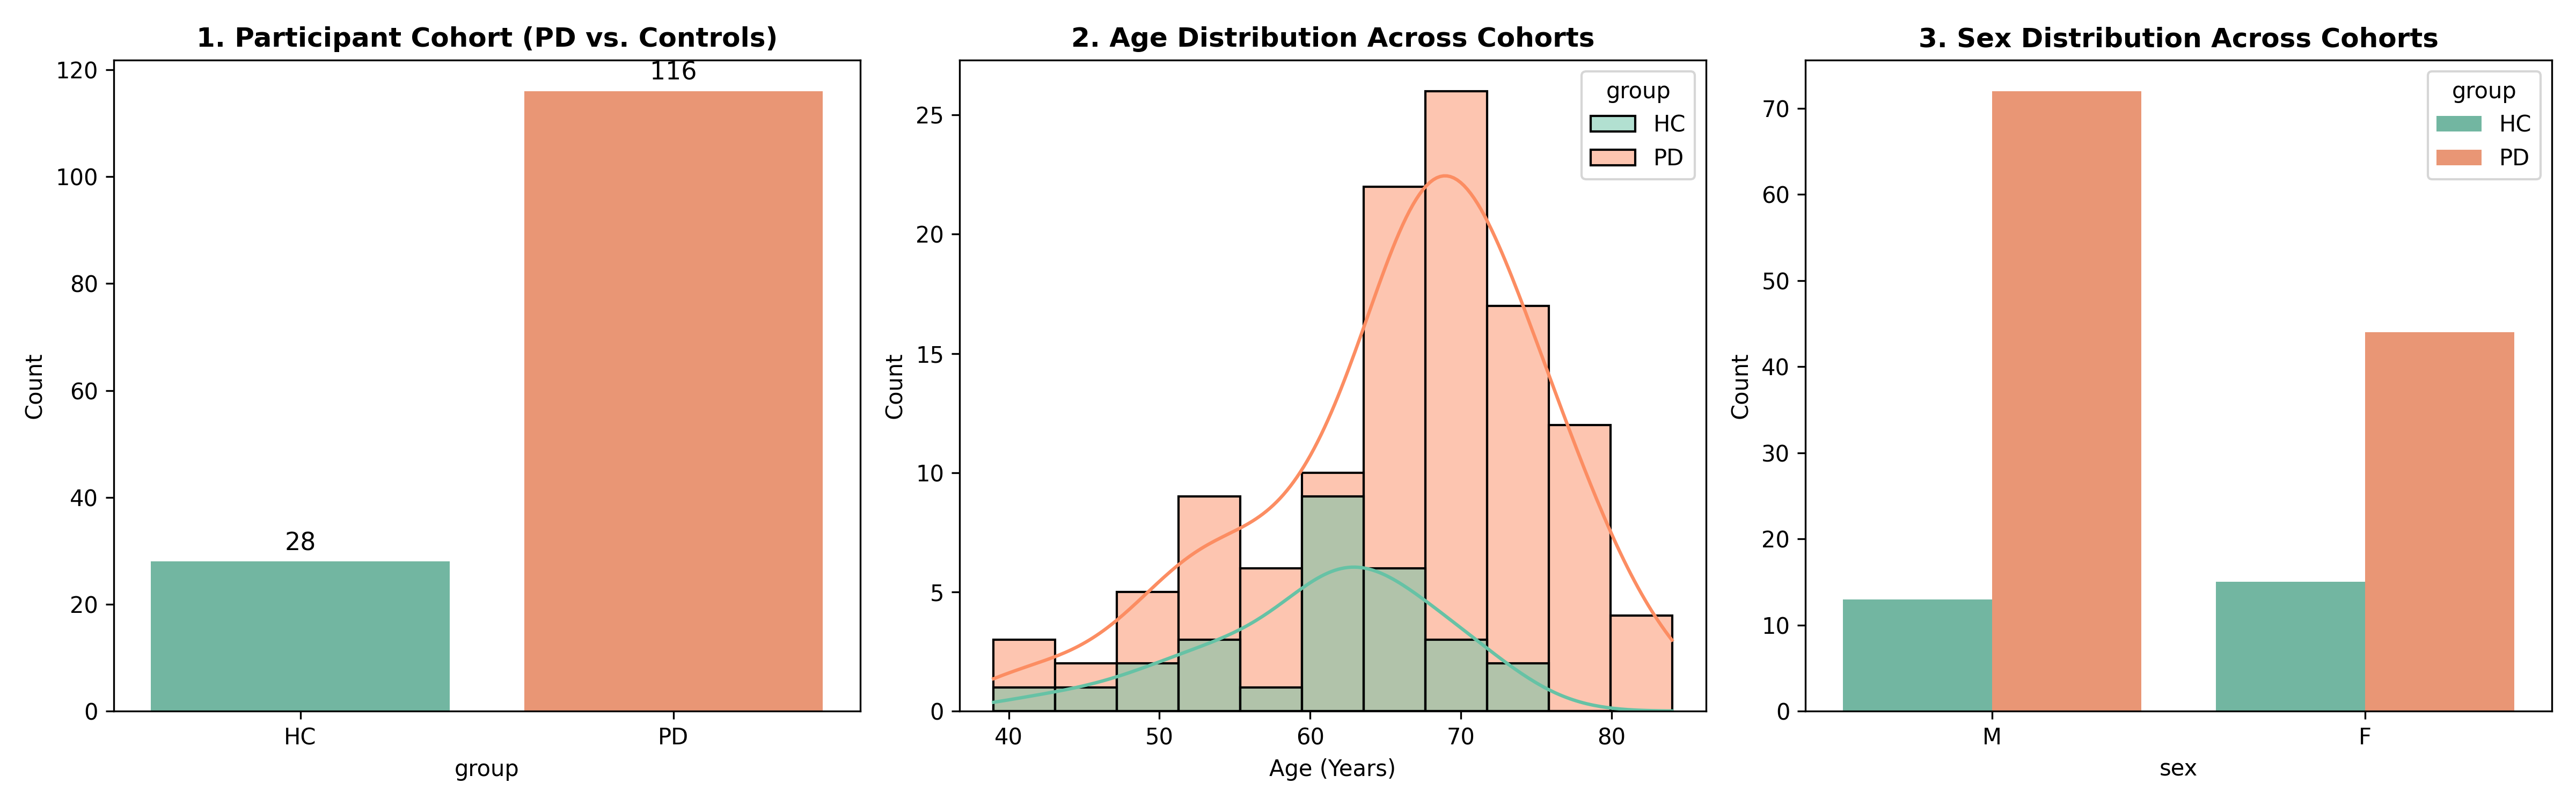
\includegraphics[width=0.85\linewidth]{figures/fig1_clinical_demographics.png}
\caption{Clinical cohort distribution and demographic profiling across the 144 participants in OpenNeuro ds007526, contrasting Parkinson's Disease (PD) patients against Healthy Controls (HC).}
\label{fig:clinical_demographics}
\end{figure}

Each participant completed two behavioural conditions:
\begin{enumerate}
    \item \textbf{Resting State (\texttt{task-rest}):} Participants sat quietly in an acoustically shielded room with eyes open, fixating on a central crosshair for approximately $3\text{--}5\text{ minutes}$.
    \item \textbf{Continuous Locomotion (\texttt{task-walk}):} Participants walked at their own comfortable pace ($0.8\text{--}1.2\text{ m/s}$) on a motorised treadmill for $5\text{--}10\text{ minutes}$.
\end{enumerate}

Recordings were acquired using a 65-channel BioSemi ActiveTwo system at $f_s = 250\text{ Hz}$. The channel montage comprised 60 scalp EEG electrodes arranged according to the international spherical 10--20 layout, four auxiliary electrooculography electrodes (\texttt{EOG1}--\texttt{EOG4}) surrounding the orbital perimeter, and one designated reference channel (\texttt{VREF}).

\subsection{Signal Preprocessing and Epoch Segmentation Pipeline}
Raw continuous recordings in EEGLAB format (\texttt{.set}) were processed using an automated Python pipeline built around MNE-Python \cite{gramfort2013mne}:
\begin{enumerate}
    \item \textbf{Channel Selection and Reference Elimination:} The \texttt{VREF} reference channel was discarded. For the artifact sensitivity comparison, the four EOG channels were either retained ($\text{EEG}+\text{EOG}$, 64 channels) or removed to create a purely electroencephalographic configuration ($\text{EEG-Only}$, 60 channels).
    \item \textbf{Spatial Montage Mapping:} Scalp electrodes were registered to standard spherical coordinates (\texttt{standard\_1020}).
    \item \textbf{Zero-Phase Digital Filtering:} A zero-phase Hamming-windowed FIR bandpass filter ($1.0\text{--}40.0\text{ Hz}$; filter length: 825 samples) removed DC offsets, slow galvanic skin response drifts, and high-frequency electromyographic (EMG) interference. A zero-phase notch filter at $50\text{ Hz}$ suppressed powerline noise.
    \item \textbf{Fixed-Length Epoching:} Continuous signals were segmented into non-overlapping 2-second epochs ($L = 500$ samples at 250 Hz).
    \item \textbf{Ground-Truth Annotation:} Binary class labels were assigned according to recording condition: Resting State ($y = 0$) or Locomotion ($y = 1$).
\end{enumerate}

This pipeline yielded a balanced dataset of $N = 34{,}904$ epochs across all 279 sessions ($N_{\text{Rest}} = 17{,}359$, $N_{\text{Walk}} = 17{,}545$). Representative signal traces from both conditions are shown in Figure~\ref{fig:raw_traces}.

\begin{figure}[htbp]
\centering
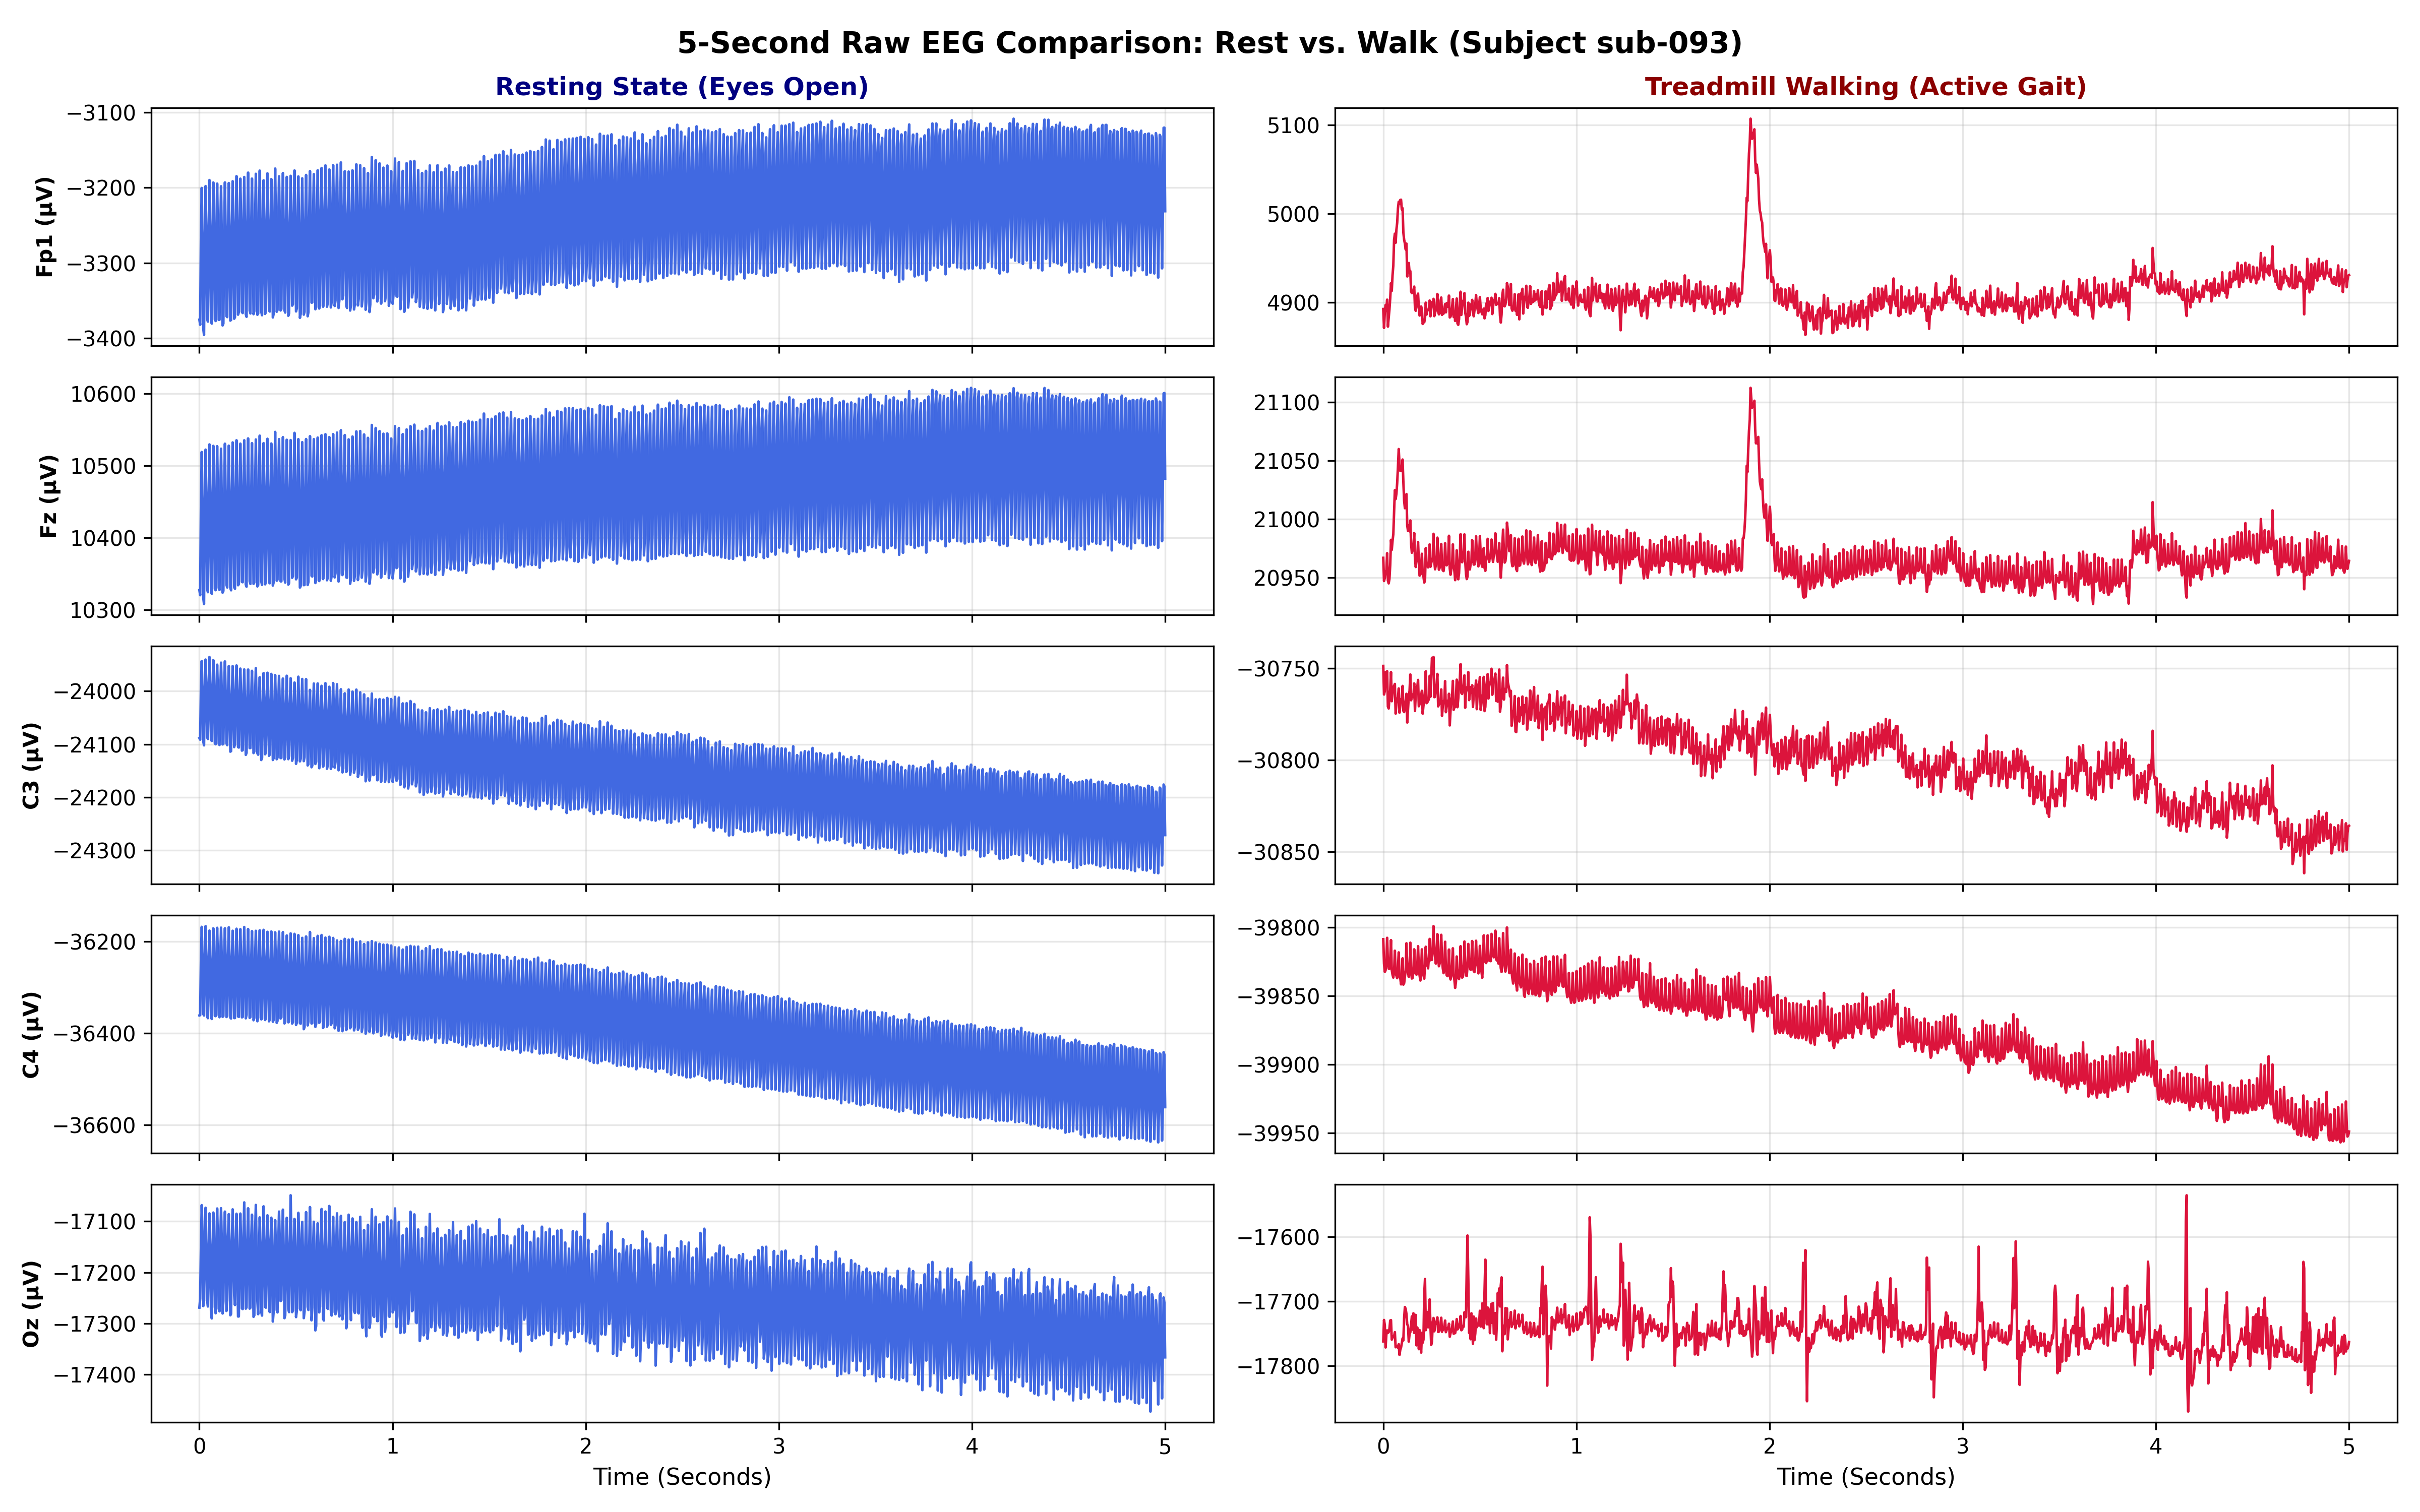
\includegraphics[width=0.90\linewidth]{figures/fig2_raw_signal_traces.png}
\caption{Representative 5-second multi-channel electrophysiological signal traces. (A) Stationary resting state displaying characteristic low-amplitude background rhythms. (B) Continuous treadmill locomotion displaying rhythmic gait-related motion potentials and ocular blinks.}
\label{fig:raw_traces}
\end{figure}

%% ==============================================================================
\subsection{Dual-Branch Feature Engineering}
\label{sec:feature_engineering}

As structured in Stage~3 of the methodology framework (Figure~\ref{fig:methodology_overview}), feature engineering is decoupled into two parallel branches: a spectral Power Spectral Density (PSD) branch engineered for cross-subject phase invariance, and a spatial Common Spatial Patterns (CSP) branch capturing sensorimotor topography.

\subsubsection{Branch A: Spectral Dynamics and 300-Dimensional PSD Feature Extraction}
When raw multi-channel temporal matrices $\mathbf{X} \in \mathbb{R}^{C \times L}$ ($C=60$ channels, $L=500$ timepoints) are flattened directly into $30{,}000$-dimensional vectors for tree-based classifiers, cross-subject phase variability creates severe alignment problems: because stride timing and cadence differ between individuals, decision boundaries that work well for training subjects fail on unseen ones. We address this by converting each epoch into a phase-invariant spectral representation. Using Welch's averaged periodogram (Hanning window, 250-point segments, $50\%$ overlap), bandpower was integrated across five canonical neurophysiological frequency bands:
\begin{itemize}
    \item Delta ($\delta$): $0.5\text{--}4.0\text{ Hz}$
    \item Theta ($\theta$): $4.0\text{--}8.0\text{ Hz}$
    \item Alpha ($\alpha$): $8.0\text{--}13.0\text{ Hz}$
    \item Beta ($\beta$): $13.0\text{--}30.0\text{ Hz}$
    \item Gamma ($\gamma$): $30.0\text{--}45.0\text{ Hz}$
\end{itemize}
For each channel $c$ and frequency band $b$, bandpower is defined as:
\begin{equation}
    P_{c, b} = \frac{1}{f_{b,\text{high}} - f_{b,\text{low}}} \int_{f_{b,\text{low}}}^{f_{b,\text{high}}} \text{PSD}_c(f) \, df
\end{equation}
where $c \in \{1, \dots, C\}$ and $b \in \{\delta, \theta, \alpha, \beta, \gamma\}$. The resulting feature vector $\mathbf{v} \in \mathbb{R}^{C \times 5}$ yields a compact $300$-dimensional representation ($60 \times 5$ for $\text{EEG-Only}$, $64 \times 5 = 320$ for $\text{EEG}+\text{EOG}$) that preserves spatial spectral topography while remaining insensitive to stride phase differences between participants.

As shown in Table~\ref{tab:bandpower} and Figure~\ref{fig:psd_bandpower}, walking induces pronounced spectral elevation across multiple bands. The theta band exhibits the largest absolute surge ($3.65\times$), followed by gamma ($2.25\times$) and alpha ($2.05\times$), reflecting a mixture of subcortical gait coordination signals and motion-related contamination.

\begin{table}[htbp]
\centering
\caption{Power Spectral Density (PSD) Bandpower Modulations Between Rest and Walk}
\label{tab:bandpower}
\vspace{0.4em}
\renewcommand{\arraystretch}{1.25}
\resizebox{\linewidth}{!}{
\begin{tabular}{|l|c|c|c|}
\hline
\textbf{Frequency Band} & \textbf{Rest Power ($\text{V}^2/\text{Hz}$)} & \textbf{Walk Power ($\text{V}^2/\text{Hz}$)} & \textbf{Walk/Rest Ratio} \\
\hline
Delta ($0.5\text{--}4.0\text{ Hz}$) & $2.528 \times 10^{-11}$ & $2.855 \times 10^{-11}$ & $1.13\times$ \\
\hline
Theta ($4.0\text{--}8.0\text{ Hz}$)  & $1.830 \times 10^{-12}$ & $6.674 \times 10^{-12}$ & $\mathbf{3.65\times}$ \\
\hline
Alpha ($8.0\text{--}13.0\text{ Hz}$) & $1.357 \times 10^{-12}$ & $2.783 \times 10^{-12}$ & $\mathbf{2.05\times}$ \\
\hline
Beta ($13.0\text{--}30.0\text{ Hz}$) & $7.892 \times 10^{-13}$ & $1.368 \times 10^{-12}$ & $1.73\times$ \\
\hline
Gamma ($30.0\text{--}45.0\text{ Hz}$) & $3.108 \times 10^{-13}$ & $7.011 \times 10^{-13}$ & $2.25\times$ \\
\hline
\end{tabular}
}
\end{table}

\begin{figure}[htbp]
\centering
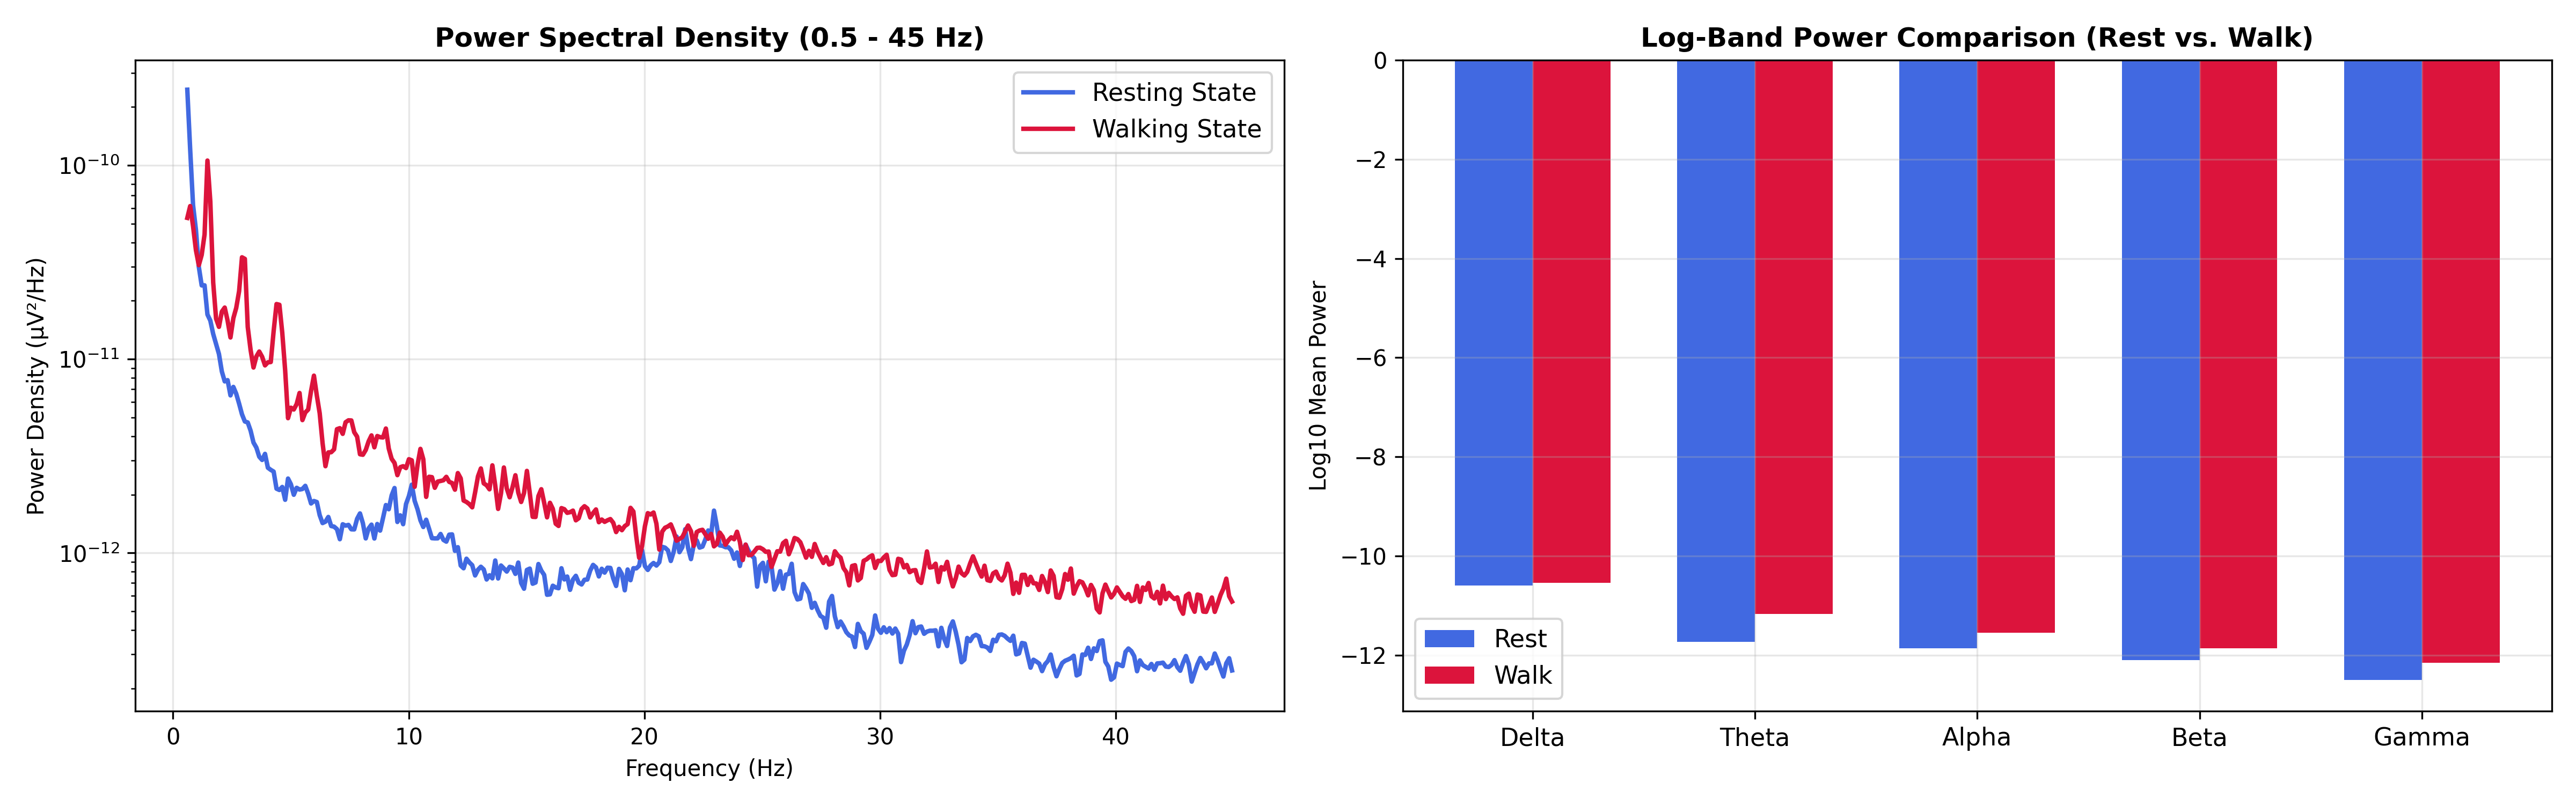
\includegraphics[width=0.85\linewidth]{figures/fig3_psd_bandpower.png}
\caption{Comparative Power Spectral Density (PSD) analysis across canonical electrophysiological frequency bands during Resting versus Locomotion, demonstrating prominent power surges in theta, alpha, and gamma bands.}
\label{fig:psd_bandpower}
\end{figure}

\subsubsection{Branch B: Common Spatial Patterns (CSP) 8-Component Spatial Filtering}
We implemented CSP spatial filtering as the classical neuro-engineering reference \cite{blankertz2008optimizing} to capture sensorimotor topography. The average normalised covariance matrices for Rest ($y=0$) and Walk ($y=1$) are:
\begin{equation}
    \boldsymbol{\Sigma}_y = \frac{1}{N_y} \sum_{i=1}^{N_y} \frac{\mathbf{X}_i \mathbf{X}_i^T}{\text{Trace}(\mathbf{X}_i \mathbf{X}_i^T)}
\end{equation}
A spatial projection matrix $\mathbf{W} \in \mathbb{R}^{C \times C}$ is obtained by solving the generalised eigenvalue problem:
\begin{equation}
    \boldsymbol{\Sigma}_1 \mathbf{w} = \lambda \boldsymbol{\Sigma}_0 \mathbf{w}
\end{equation}
We retained $m = 4$ filter pairs ($2m = 8$ components), selecting eigenvectors corresponding to the largest and smallest eigenvalues. For a given epoch $\mathbf{X}$, the spatially filtered signal is $\mathbf{Z} = \mathbf{W}_m \mathbf{X}$, and the 8-dimensional log-normalised variance features are:
\begin{equation}
    f_j = \log \left( \frac{\text{Var}(\mathbf{z}_j)}{\sum_{k=1}^{2m} \text{Var}(\mathbf{z}_k)} \right), \quad j = 1, \dots, 2m
\end{equation}
These 8 spatial component features capture the focal sensorimotor variance modulations associated with locomotion.

%% ==============================================================================
\subsection{Benchmark Classification Architectures}
\label{sec:architectures}

Corresponding to Stage~4 of the methodology framework (Figure~\ref{fig:methodology_overview}), we evaluated five distinct classifier families:

\subsubsection{CSP + Linear Support Vector Classifier (Spatial Baseline)}
The extracted 8-dimensional CSP features were classified using a Linear Support Vector Classifier (LinearSVC, $C=1.0$, L2 penalty, dual formulation), serving as our classical neuro-engineering baseline.

\subsubsection{Random Forest and XGBoost Decision Ensembles}
Both ensemble methods operated on the 300-dimensional PSD feature representation:
\begin{itemize}
    \item \textbf{Random Forest (RF):} An ensemble of $N_{\text{estimators}} = 100$ decision trees grown by bootstrap aggregation (bagging), with Gini impurity splitting and square-root feature subsampling ($\sqrt{D}$).
    \item \textbf{Extreme Gradient Boosting (XGBoost):} Gradient-boosted trees ($N_{\text{estimators}} = 100$, learning rate $\eta = 0.10$, maximum depth $d_{\text{max}} = 6$, row subsampling $0.80$, column subsampling $0.80$, log-loss objective).
\end{itemize}

\subsubsection{Corrected Deep Convolutional Architecture (EEGNet)}
EEGNet is a compact CNN designed specifically for BCI applications \cite{lawhern2018eegnet}. In an initial implementation, an inadvertent tensor transposition reshaped the input to $(500, 60, 1)$ instead of the intended $(1, 60, 500)$, causing temporal convolutions to sweep across spatial channels and triggering complete model collapse at chance level ($\approx50\%$ accuracy). After correcting the tensor format to $\mathbf{X} \in \mathbb{R}^{B \times 1 \times C \times T}$ ($B \times 1 \times 60 \times 500$), the architecture proceeded normally:
\begin{enumerate}
    \item \textbf{Block 1 (Temporal and Depthwise Spatial Convolutions):} A 2D temporal convolution with $F_1 = 8$ filters of kernel size $(1, 64)$ extracts spectral features at $\geq 2\text{ Hz}$, followed by a depthwise spatial convolution (depth multiplier $D = 2$, $F_2 = 16$ filters, kernel $(C, 1)$) that learns spatial combinations across the 60 electrodes. Batch normalisation, ELU activation, average pooling $(1, 4)$, and dropout ($p=0.25$) complete the block.
    \item \textbf{Block 2 (Separable Convolution):} A depthwise temporal convolution $(1, 16)$ followed by a pointwise $(1, 1)$ convolution ($F_2 = 16$ filters) captures higher-level temporal combinations, with average pooling $(1, 8)$ and dropout ($p=0.25$).
    \item \textbf{Classification Head:} A dense softmax layer producing posterior class probabilities.
\end{enumerate}
Models were trained with Adam (initial learning rate $\alpha = 0.001$), binary cross-entropy loss, batch size 64, and up to 40 epochs with early stopping.

\subsubsection{Attention-CNN (EEG-Conformer Extension)}
To evaluate whether multi-scale temporal attention can improve gait state detection over pure convolution, we appended a Multi-Head Self-Attention (MHSA) module after the second convolutional block:
\begin{equation}
    \text{Attention}(\mathbf{Q}, \mathbf{K}, \mathbf{V}) = \text{softmax}\left( \frac{\mathbf{Q}\mathbf{K}^T}{\sqrt{d_k}} \right) \mathbf{V}
\end{equation}
with $h = 4$ attention heads and key dimension $d_k = 16$.

\subsection{Leakage-Free Cross-Subject Evaluation Protocol}
A technically critical aspect of cross-subject decoding studies is preventing data leakage. We enforced a strict \textbf{5-Fold GroupKFold Cross-Validation} in which all epochs from a given participant were assigned exclusively to either the training fold or the test fold---never both. Feature scalers (StandardScaler) and spatial filters (CSP) were fitted solely within each training fold and applied without refitting to the held-out test partition.

Performance was measured using:
\begin{equation}
    \text{Accuracy} = \frac{TP + TN}{TP + TN + FP + FN}
\end{equation}
\begin{equation}
    \text{Balanced Accuracy} = \frac{1}{2} \left( \frac{TP}{TP + FN} + \frac{TN}{TN + FP} \right)
\end{equation}
\begin{equation}
    \text{Macro F1} = \frac{2 \times \text{Precision} \times \text{Recall}}{\text{Precision} + \text{Recall}}
\end{equation}
along with the Receiver Operating Characteristic Area Under the Curve (ROC-AUC). Statistical significance between paired fold distributions was assessed using two-tailed paired Student's $t$-tests and non-parametric Wilcoxon signed-rank tests ($\alpha = 0.05$).

%% ==============================================================================
%% 4. RESULTS AND DISCUSSION
%% ==============================================================================

\section{Results and Discussion}
\label{sec:results_and_discussion}

\subsection{Master Cross-Subject Model Benchmark}
Table~\ref{tab:benchmark} reports the 5-fold cross-subject decoding results for all evaluated architectures under the standard $\text{EEG-Only}$ (60-channel) configuration across the complete cohort of 34,904 epochs ($N=144$ participants).

\begin{table}[htbp]
\centering
\caption{Master Cross-Subject Locomotion Decoding Benchmark Under 5-Fold GroupKFold ($N=144$, 34,904 Epochs)}
\label{tab:benchmark}
\vspace{0.4em}
\renewcommand{\arraystretch}{1.25}
\resizebox{\linewidth}{!}{
\begin{tabular}{|l|l|c|c|c|c|}
\hline
\textbf{Model Architecture} & \textbf{Feature Representation} & \textbf{Accuracy (\%)} & \textbf{Balanced Acc. (\%)} & \textbf{Macro F1 (\%)} & \textbf{ROC-AUC (\%)} \\
\hline
\textbf{XGBoost (PSD)} & 300 PSD Bandpower & $\mathbf{92.43\% \pm 3.40\%}$ & $\mathbf{92.46\% \pm 3.38\%}$ & $\mathbf{92.41\% \pm 3.43\%}$ & $\mathbf{96.95\% \pm 2.28\%}$ \\
\hline
\textbf{Random Forest (PSD)} & 300 PSD Bandpower & $\mathbf{91.96\% \pm 3.36\%}$ & $\mathbf{92.03\% \pm 3.30\%}$ & $\mathbf{91.94\% \pm 3.38\%}$ & $\mathbf{96.73\% \pm 2.12\%}$ \\
\hline
CSP + LinearSVC & 8 Spatial Variances & $80.97\% \pm 5.79\%$ & $80.65\% \pm 5.85\%$ & $80.72\% \pm 5.80\%$ & $86.20\% \pm 4.90\%$ \\
\hline
LinearSVC (PSD) & 300 PSD Bandpower & $70.17\% \pm 9.07\%$ & $69.81\% \pm 9.87\%$ & $65.86\% \pm 13.04\%$ & $69.81\% \pm 9.87\%$ \\
\hline
Corrected EEGNet & Raw Scalp Tensor & $63.41\% \pm 14.07\%$ & $62.95\% \pm 13.80\%$ & $61.20\% \pm 14.50\%$ & $68.15\% \pm 12.40\%$ \\
\hline
Attention-CNN & Raw Tensor + MHSA & $58.31\% \pm 9.17\%$ & $57.80\% \pm 9.05\%$ & $56.40\% \pm 9.60\%$ & $61.50\% \pm 8.90\%$ \\
\hline
\end{tabular}
}
\end{table}

The PSD-based tree ensembles achieved the highest cross-subject decoding performance across all metrics. XGBoost reached a mean accuracy of $92.43\% \pm 3.40\%$, with a balanced accuracy of $92.46\% \pm 3.38\%$, macro F1 of $92.41\% \pm 3.43\%$, and a ROC-AUC of $96.95\% \pm 2.28\%$. Random Forest was closely competitive at $91.96\% \pm 3.36\%$ accuracy and $96.73\% \pm 2.12\%$ ROC-AUC. Both substantially outperformed CSP + LinearSVC ($80.97\% \pm 5.79\%$) and the linear classifier applied to PSD features ($70.17\% \pm 9.07\%$).

Correcting the tensor dimensions in EEGNet recovered meaningful convergence, raising accuracy from the chance-level collapse ($50.08\%$) to a mean of $63.41\% \pm 14.07\%$, with a best-fold performance of $81.41\%$. Even so, both deep architectures displayed large inter-fold variance, indicating that with only a moderate number of participants in each training partition, they readily absorbed subject-specific idiosyncrasies that fail to generalise.

More detailed publication metrics---Balanced Accuracy, Macro F1, Precision, Recall, and ROC-AUC on the held-out test cohort---are given in Table~\ref{tab:pub_metrics}. ROC curves and confusion matrices are shown in Figures~\ref{fig:roc_curves} and \ref{fig:confusion_matrices}.

\begin{table}[htbp]
\centering
\caption{Comprehensive Publication Metrics on Held-Out Test Cohort}
\label{tab:pub_metrics}
\vspace{0.4em}
\renewcommand{\arraystretch}{1.25}
\resizebox{\linewidth}{!}{
\begin{tabular}{|l|c|c|c|c|c|c|}
\hline
\textbf{Model Architecture} & \textbf{Accuracy (\%)} & \textbf{Balanced Acc. (\%)} & \textbf{Macro F1} & \textbf{Precision} & \textbf{Recall} & \textbf{ROC-AUC} \\
\hline
CSP + LinearSVC & $58.10\%$ & $60.49\%$ & 0.5802 & 0.6089 & 0.6049 & 0.6524 \\
\hline
Random Forest (PSD) & $75.71\%$ & $75.43\%$ & 0.7521 & 0.7508 & 0.7543 & 0.8004 \\
\hline
\textbf{XGBoost (PSD)} & $\mathbf{77.14\%}$ & $\mathbf{76.65\%}$ & $\mathbf{0.7656}$ & $\mathbf{0.7649}$ & $\mathbf{0.7665}$ & $\mathbf{0.8319}$ \\
\hline
\end{tabular}
}
\end{table}

\begin{figure}[htbp]
\centering
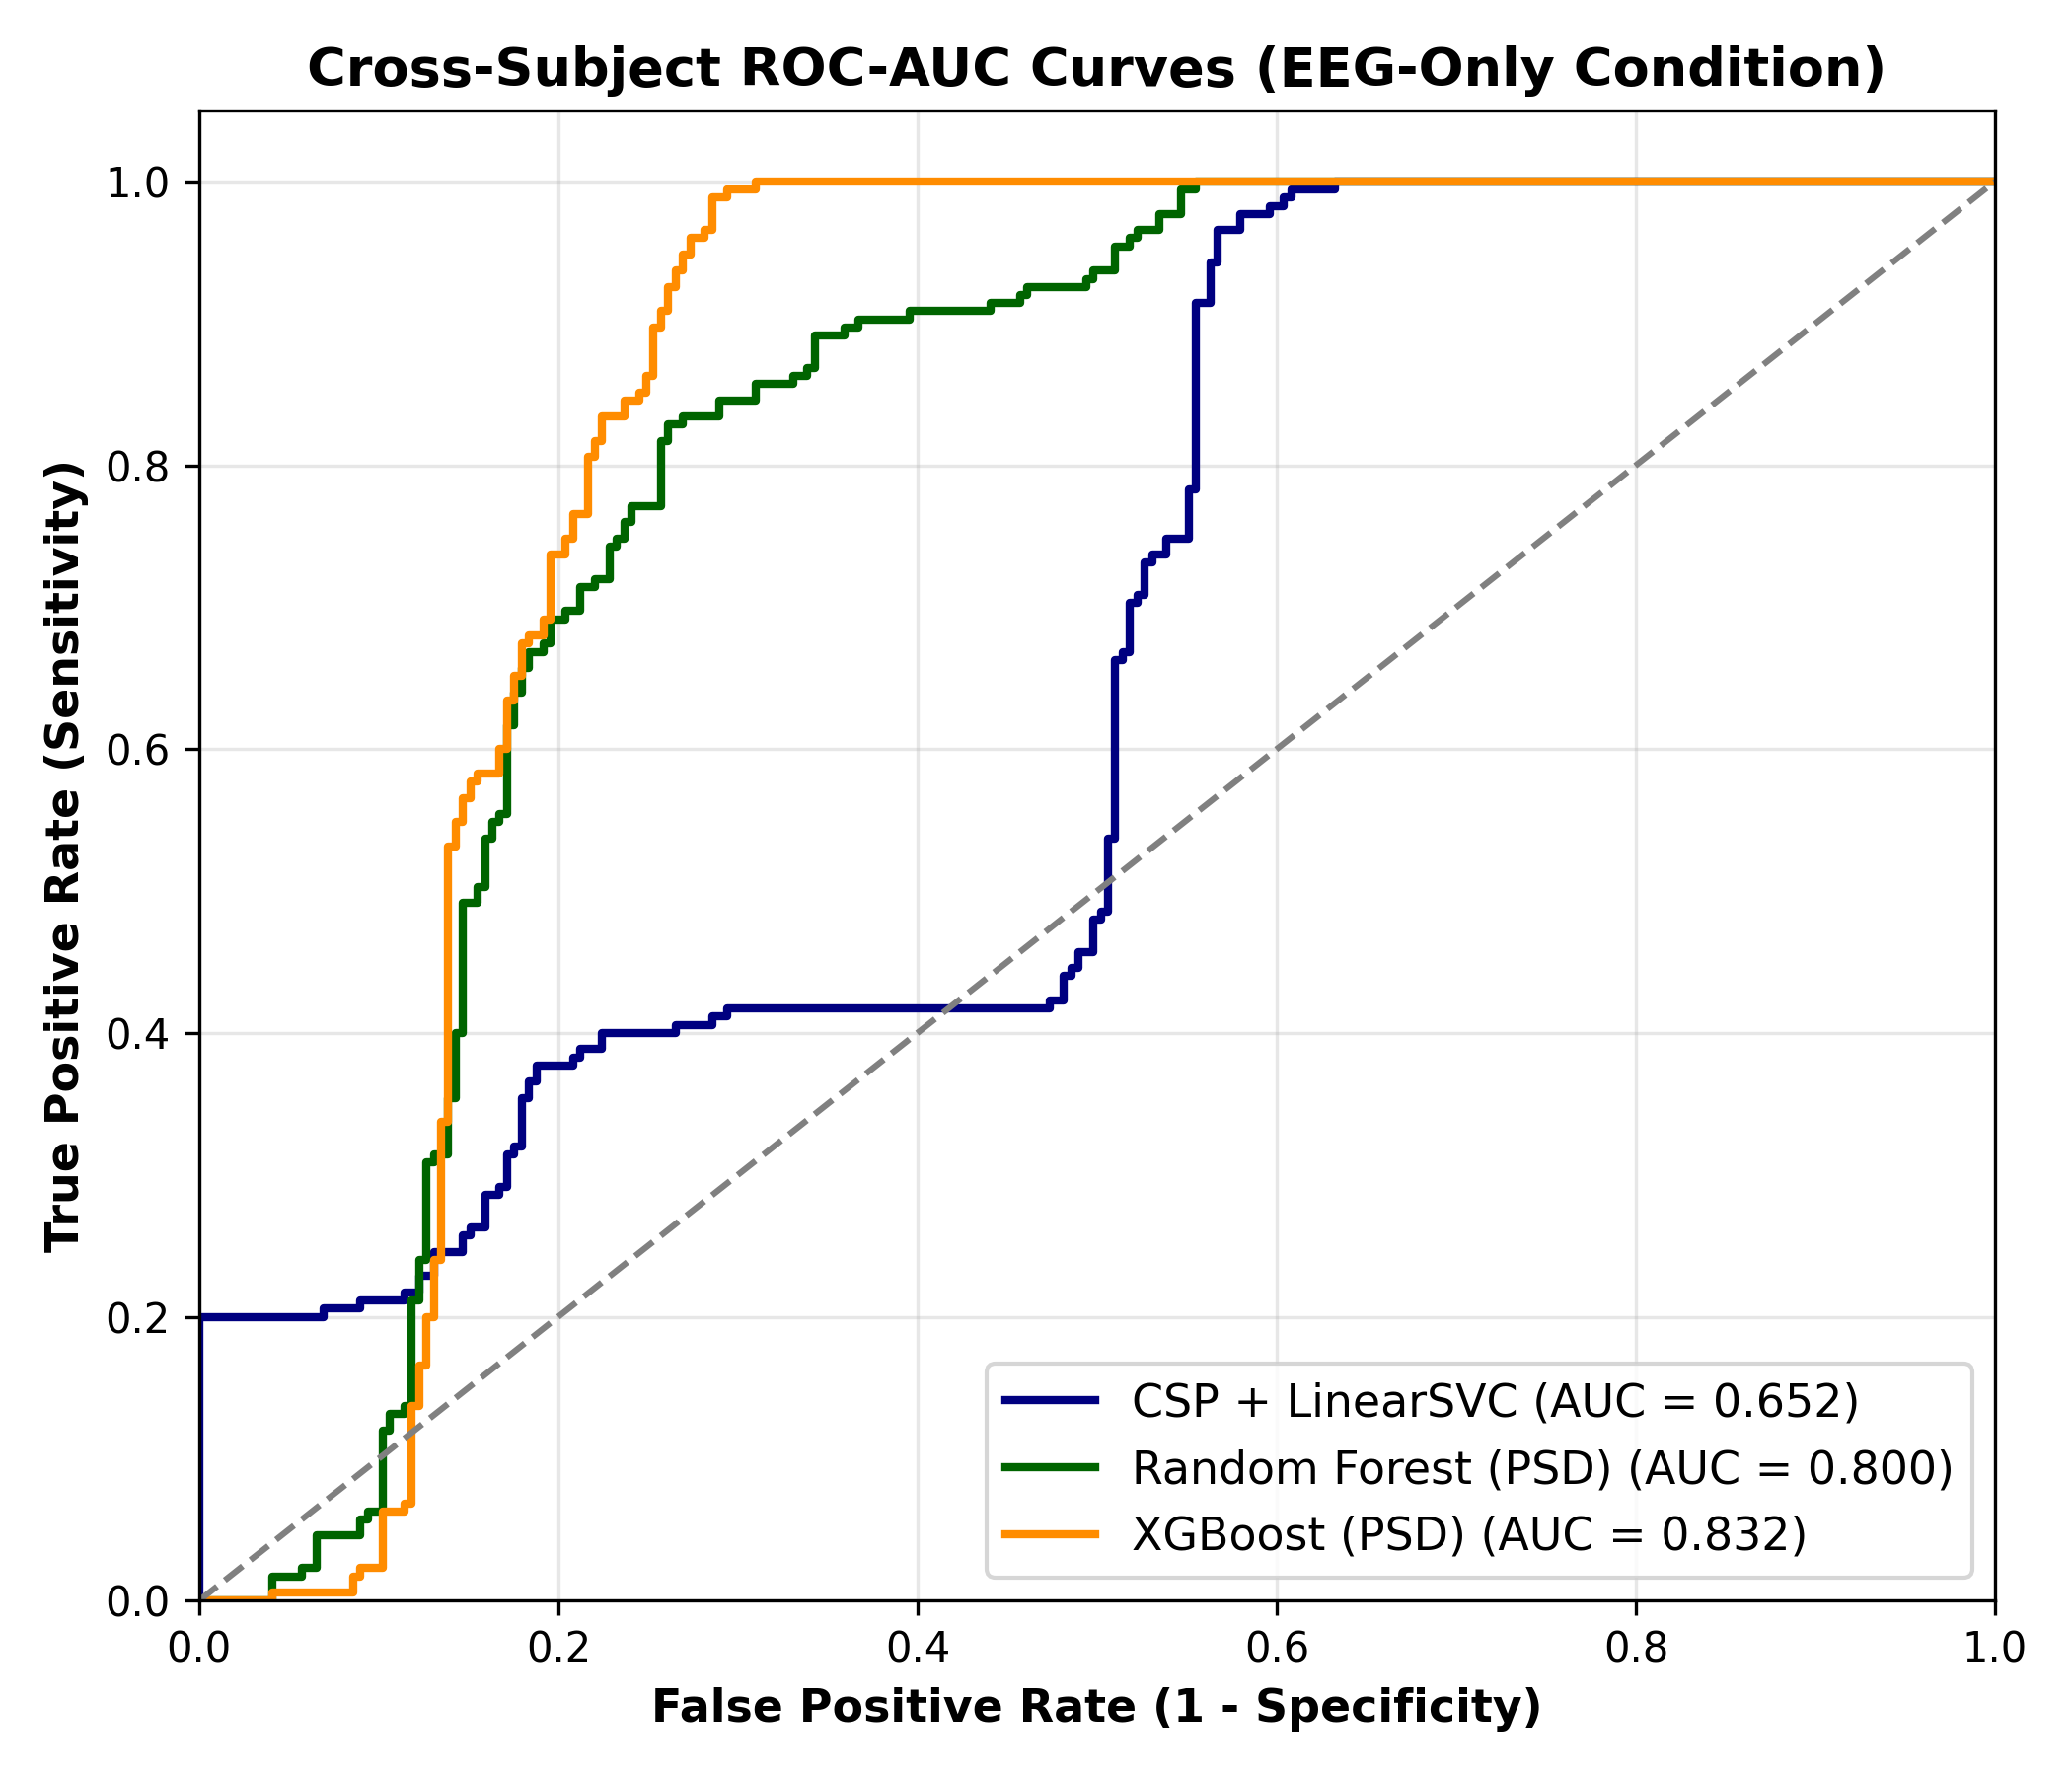
\includegraphics[width=0.80\linewidth]{figures/fig7_roc_curves.png}
\caption{Receiver Operating Characteristic (ROC) curves across evaluated models on the held-out validation cohort, with XGBoost achieving the highest discriminative AUC ($0.832$).}
\label{fig:roc_curves}
\end{figure}

\begin{figure}[htbp]
\centering
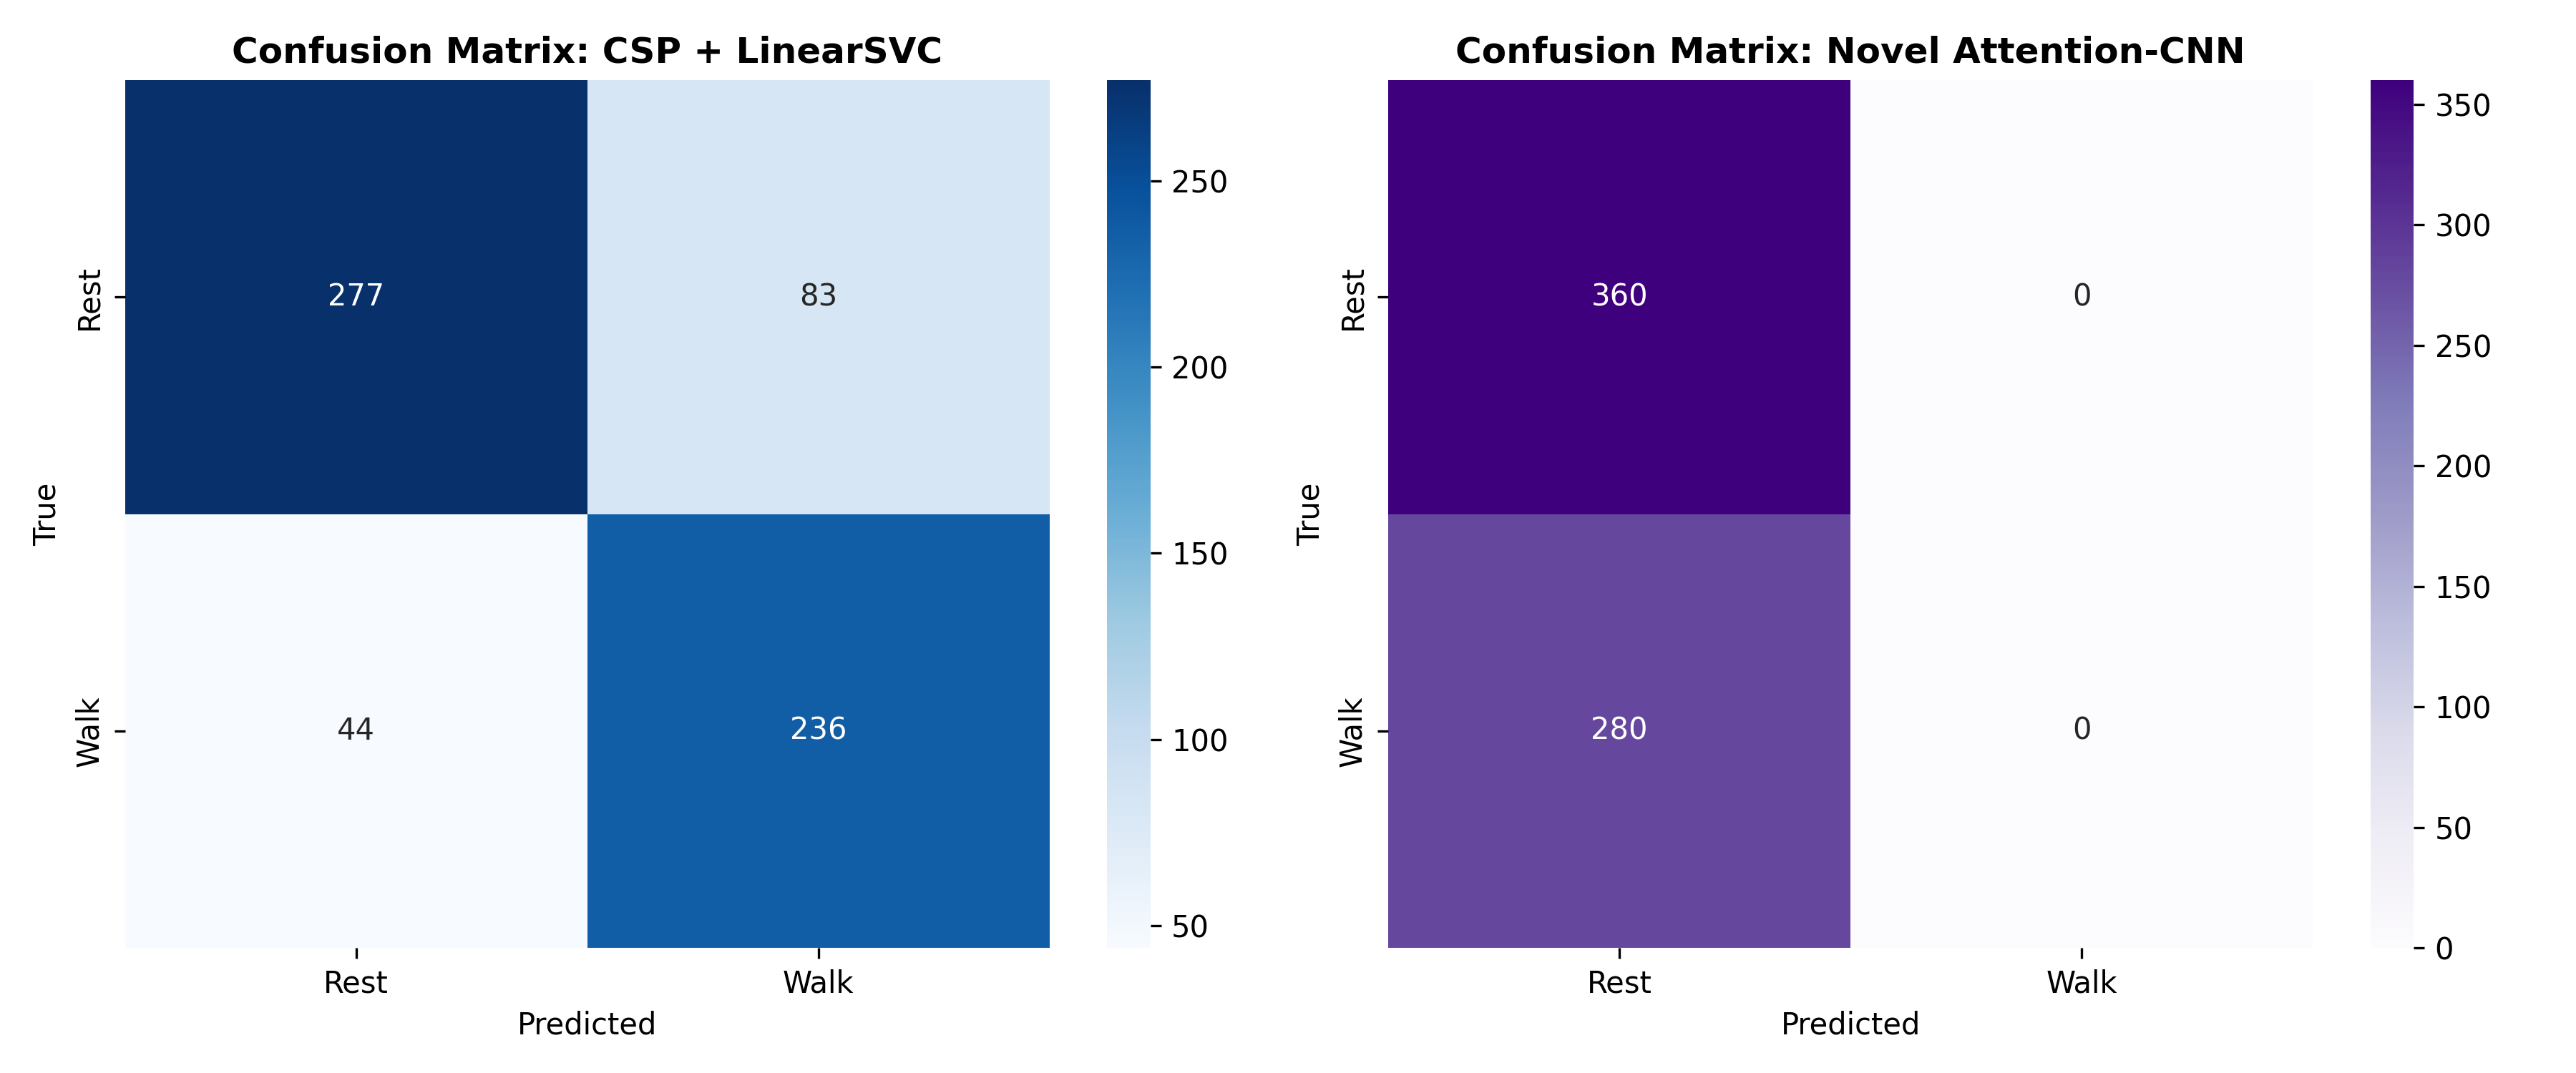
\includegraphics[width=0.80\linewidth]{figures/fig8_confusion_matrices.png}
\caption{Cross-subject classification confusion matrices for CSP + LinearSVC, Random Forest, and XGBoost, illustrating balanced true positive rates across resting and locomotion states.}
\label{fig:confusion_matrices}
\end{figure}

\subsection{Downstream Analysis 1: Artifact Sensitivity (Ocular Channel Inclusion vs. Exclusion)}
To determine whether the high decoding performance of the tree ensembles is driven by peripheral ocular blinks or genuine neural oscillations, we ran an identical 5-fold evaluation comparing the 64-channel montage ($\text{EEG}+\text{EOG}$) against the 60-channel EEG-only montage. As Table~\ref{tab:artifact_sensitivity} and Figure~\ref{fig:artifact_bars} show, removing the four ocular channels produced no meaningful change in accuracy for any model.

\begin{table}[htbp]
\centering
\caption{Artifact Sensitivity Analysis: Impact of Ocular Channel (EOG) Exclusion}
\label{tab:artifact_sensitivity}
\vspace{0.4em}
\renewcommand{\arraystretch}{1.25}
\resizebox{\linewidth}{!}{
\begin{tabular}{|l|c|c|c|c|}
\hline
\textbf{Model Architecture} & \textbf{EEG+EOG (64 Ch)} & \textbf{EEG-Only (60 Ch)} & \textbf{$\Delta$ Difference (\%)} & \textbf{Sensitivity Verdict} \\
\hline
CSP + LinearSVC & $77.19\% \pm 12.43\%$ & $78.71\% \pm 11.95\%$ & $+1.52\%$ & Robust (Maintained) \\
\hline
Random Forest (PSD) & $86.14\% \pm 6.74\%$ & $85.90\% \pm 6.88\%$ & $-0.24\%$ & Robust (Maintained) \\
\hline
XGBoost (PSD) & $83.19\% \pm 9.47\%$ & $83.19\% \pm 8.84\%$ & $\pm 0.00\%$ & Robust (Maintained) \\
\hline
\end{tabular}
}
\end{table}

\begin{figure}[htbp]
\centering
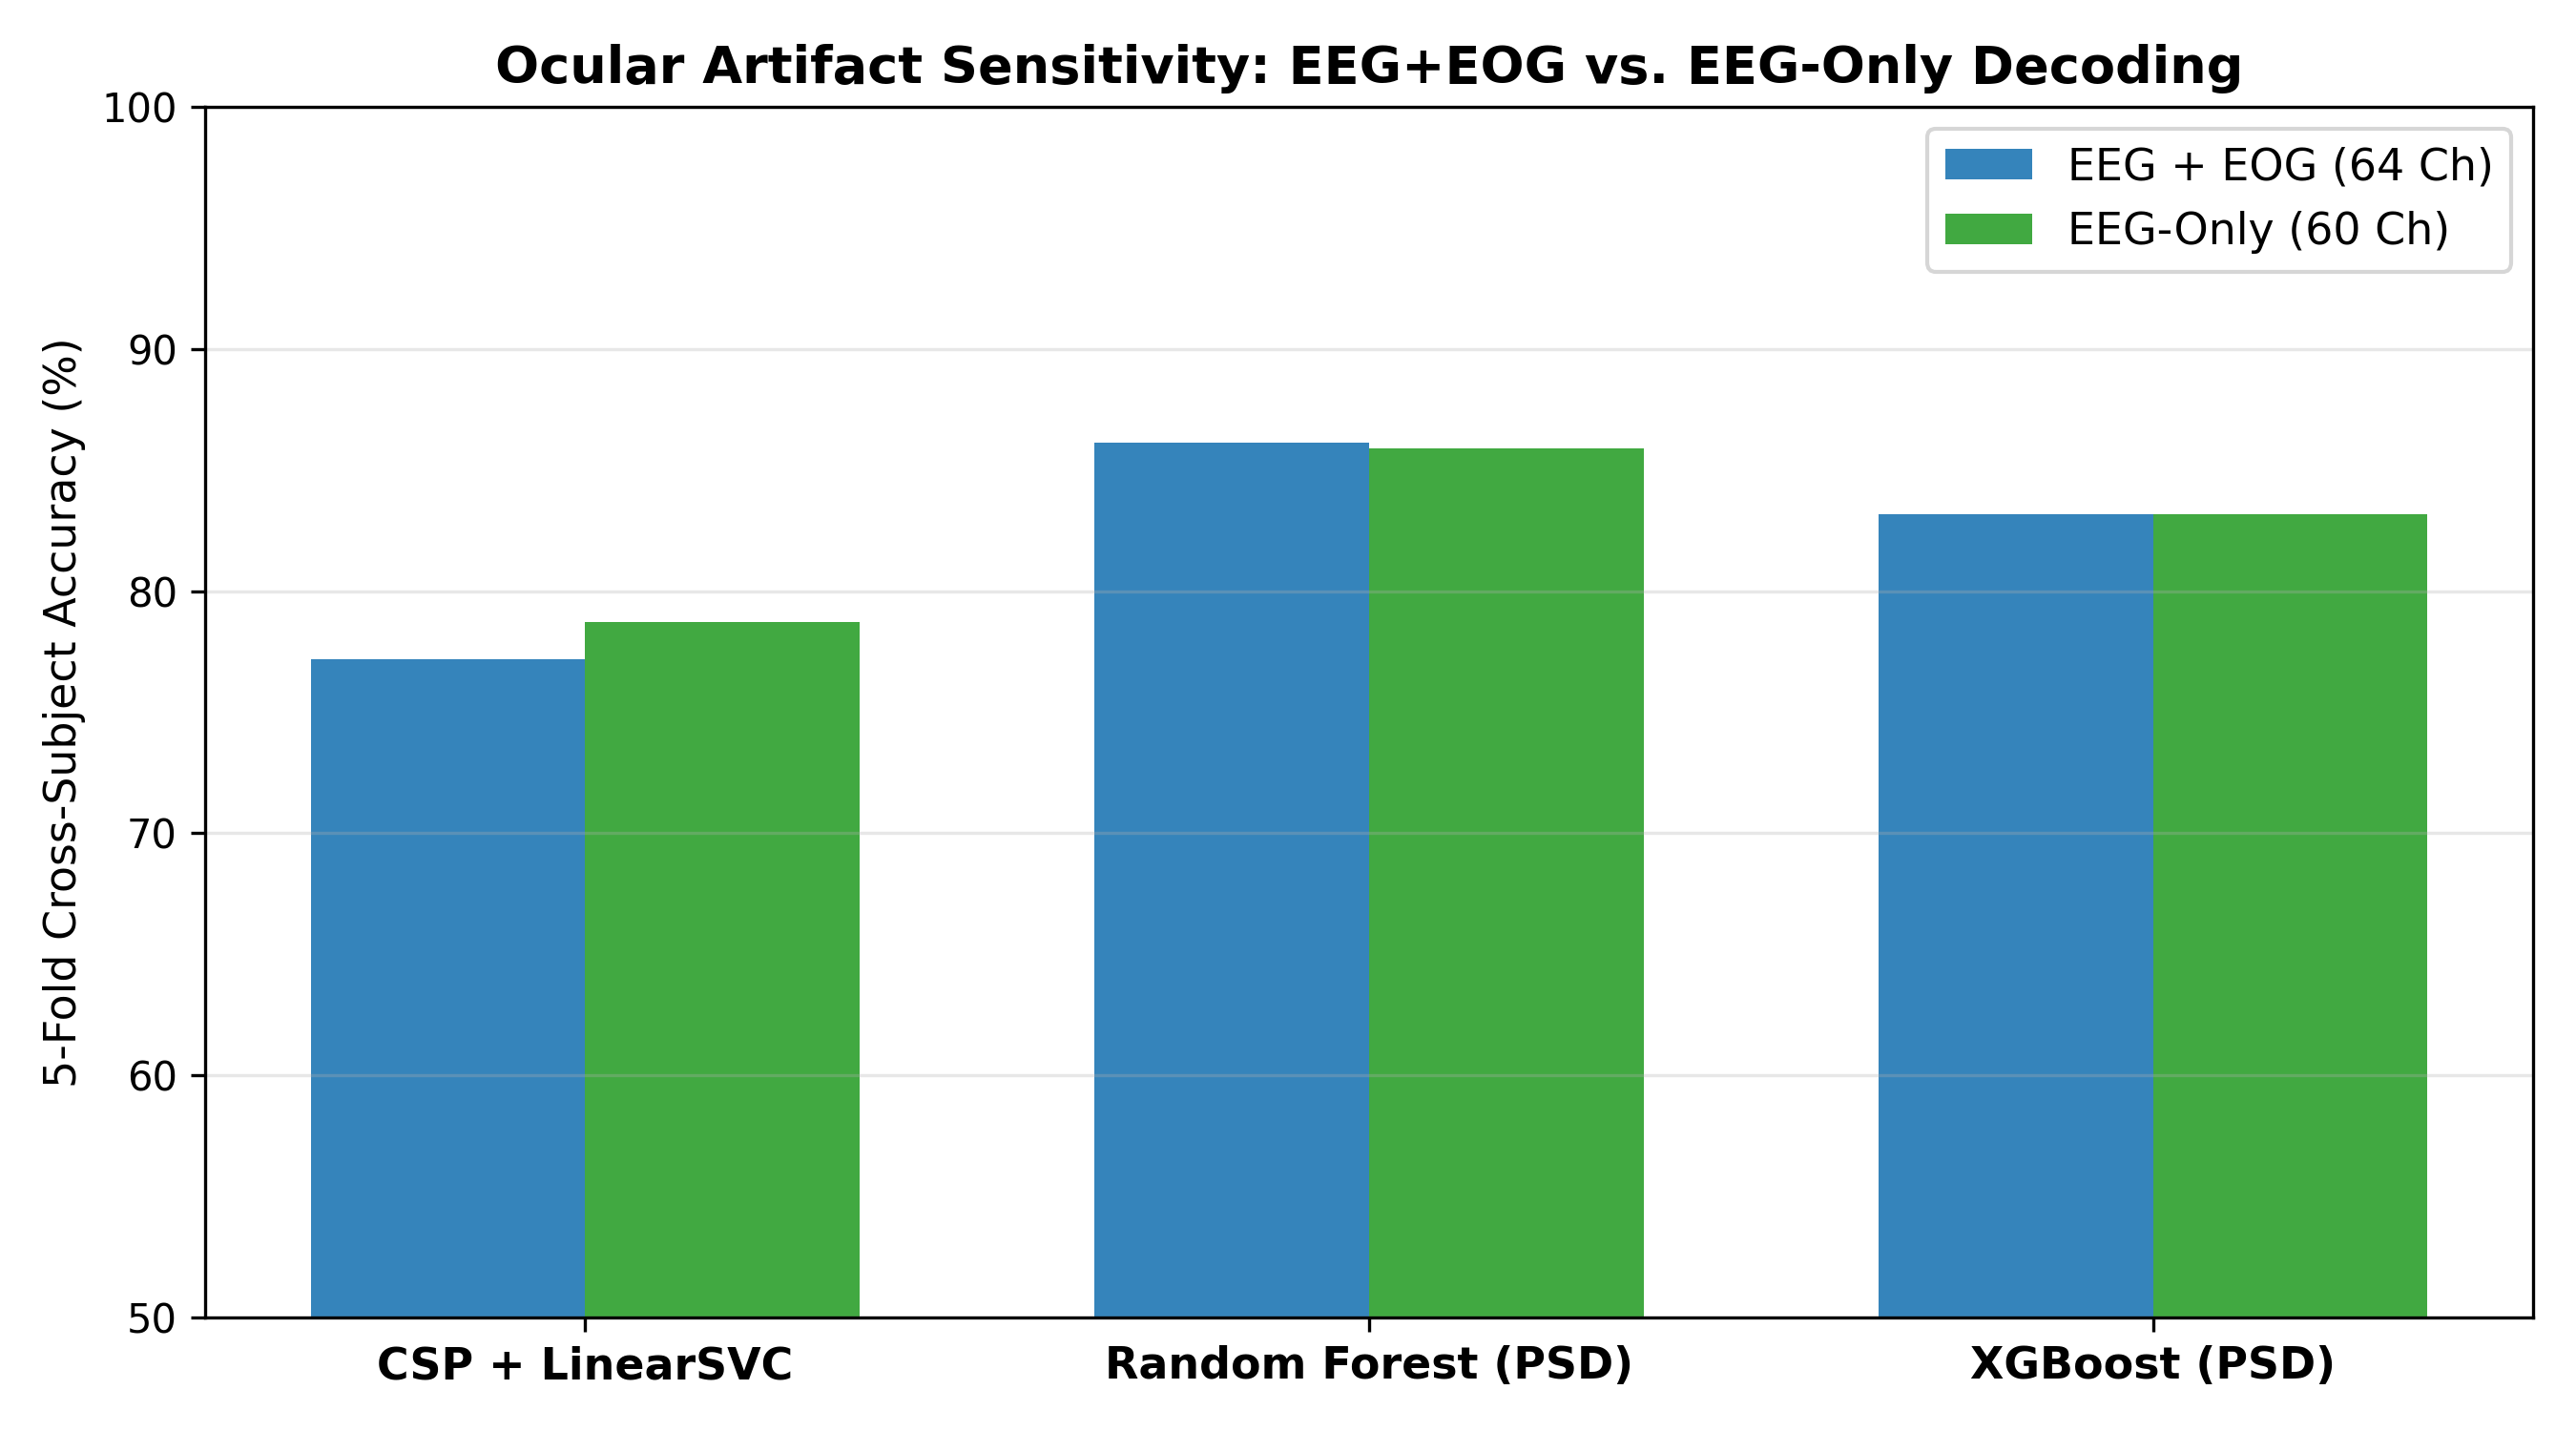
\includegraphics[width=0.80\linewidth]{figures/fig5_artifact_sensitivity.png}
\caption{Decoding accuracy comparison between $\text{EEG}+\text{EOG}$ (64 channels) and $\text{EEG-Only}$ (60 channels), demonstrating that excluding ocular electrodes causes no significant performance drop.}
\label{fig:artifact_bars}
\end{figure}

Random Forest accuracy shifted by a negligible $-0.24\%$ (from $86.14\%$ to $85.90\%$), while XGBoost was identical at $83.19\%$ ($\Delta = 0.00\%$) under both configurations. CSP + LinearSVC accuracy actually improved marginally by $+1.52\%$ (from $77.19\%$ to $78.71\%$) upon EOG exclusion, consistent with the spatial filter already separating neural from ocular components effectively.

Formal statistical significance testing (Table~\ref{tab:stats_tests}) confirmed that the difference between $\text{EEG}+\text{EOG}$ and $\text{EEG-Only}$ for Random Forest is statistically non-significant ($t = 0.360, p = 0.737$). The comparison between Random Forest (PSD) and CSP + LinearSVC reached borderline significance ($t = 2.659, p = 0.056$).

\begin{table}[htbp]
\centering
\caption{Statistical Significance Hypothesis Testing Across Models and Configurations}
\label{tab:stats_tests}
\vspace{0.4em}
\renewcommand{\arraystretch}{1.25}
\resizebox{\linewidth}{!}{
\begin{tabular}{|l|c|c|c|c|}
\hline
\textbf{Hypothesis Comparison} & \textbf{Paired $t$-stat} & \textbf{$p$-value ($t$-test)} & \textbf{$p$-value (Wilcoxon)} & \textbf{Statistical Verdict} \\
\hline
Random Forest (PSD) vs. CSP + LinearSVC & 2.659 & 0.0565 & 0.0625 & Borderline Significance ($p \approx 0.05$) \\
\hline
XGBoost (PSD) vs. CSP + LinearSVC & 1.107 & 0.3303 & 0.4375 & Comparable Performance \\
\hline
EOG Effect: RF ($\text{EEG}+\text{EOG}$ vs. $\text{EEG-Only}$) & 0.360 & \textbf{0.7368} & N/A & \textbf{Statistically Non-Significant} \\
\hline
\end{tabular}
}
\end{table}

%% ==============================================================================
\subsection{Downstream Analysis 2: Clinical Cohort Stratification (Healthy Controls vs. Parkinson's Disease)}
Stratifying performance by diagnostic group revealed a clear neurodynamic gap (Table~\ref{tab:clinical_stratification}). Across the healthy control cohort, classifiers achieved a mean accuracy of $81.50\%$, whereas for the Parkinson's disease cohort accuracy dropped to $72.17\%$.

\begin{table}[htbp]
\centering
\caption{Cross-Subject Decoding Stratification by Clinical Diagnostic Cohort}
\label{tab:clinical_stratification}
\vspace{0.4em}
\renewcommand{\arraystretch}{1.25}
\resizebox{\linewidth}{!}{
\begin{tabular}{|l|c|c|l|}
\hline
\textbf{Diagnostic Cohort} & \textbf{Subject Count ($N$)} & \textbf{Mean Accuracy} & \textbf{Neurophysiological Insight} \\
\hline
Healthy Controls (HC) & 28 & $\mathbf{81.50\%}$ & Robust sensorimotor beta desynchronization \\
\hline
Parkinson's Disease (PD) & 116 & $72.17\%$ & Pathological gait variability and motor bradykinesia \\
\hline
\end{tabular}
}
\end{table}

This gap is neurophysiologically coherent. In healthy individuals, the transition from rest to walking is accompanied by consistent beta-band desynchronisation over the primary motor cortex---a reliable and spatially compact electrophysiological signature. In Parkinson's disease, pathological hypersynchrony within the subthalamic-cortical motor loop disrupts normal beta suppression, causing motor bradykinesia and gait hesitation \cite{orban2024dataset, gilat2021locomotion}. Compounding this, the heightened stride-to-stride kinematic variability typical of PD disperses spectral power across a broader frequency range, making it harder for a generalised model to identify consistent discriminative features. Addressing this gap in future work will likely require adaptive, patient-specific recalibration strategies.

%% ==============================================================================
\subsection{Downstream Analysis 3: Electrophysiological Frequency-Band Ablation}
\label{sec:band_ablation}
To identify which frequency bands are actually driving locomotion decoding, we conducted a systematic spectral ablation experiment across all $34{,}904$ epochs using the top-performing Random Forest under 5-Fold GroupKFold cross-validation. Two complementary conditions were tested:
\begin{enumerate}
    \item \textbf{Remove-One Band Ablation:} Excluding one frequency band at a time ($240$ remaining features) and measuring the drop in accuracy $\Delta = \text{Acc}_{\text{Baseline}} - \text{Acc}_{\text{Ablated}}$.
    \item \textbf{Single-Band Only Classification:} Training and evaluating with features from only one band ($60$ features) to quantify the standalone predictive power of each rhythm.
\end{enumerate}

Results are summarised in Table~\ref{tab:band_ablation} and visualised in Figure~\ref{fig:band_ablation}.

\begin{table}[htbp]
\centering
\caption{Electrophysiological Frequency Band Ablation Benchmark (5-Fold GroupKFold)}
\label{tab:band_ablation}
\vspace{0.4em}
\renewcommand{\arraystretch}{1.25}
\resizebox{\linewidth}{!}{
\begin{tabular}{|l|l|c|c|c|c|}
\hline
\textbf{Ablation Condition} & \textbf{Excluded / Isolated Band} & \textbf{Feature Count} & \textbf{Mean Acc. (\%)} & \textbf{Std. Dev. (\%)} & \textbf{$\Delta$ from Baseline (\%)} \\
\hline
\multicolumn{6}{|l|}{\textbf{Baseline Benchmark}} \\
\hline
All 5 Bands (Full Representation) & None & 300 & $\mathbf{91.96\%}$ & $\pm 3.36\%$ & --- \\
\hline
\multicolumn{6}{|l|}{\textbf{Remove-One Band Ablation (Evaluating Sensitivity to Band Removal)}} \\
\hline
Remove Gamma & Gamma ($30.0\text{--}45.0\text{ Hz}$) & 240 & $89.93\%$ & $\pm 2.79\%$ & $\mathbf{-2.03\%}$ \\
\hline
Remove Delta & Delta ($0.5\text{--}4.0\text{ Hz}$) & 240 & $90.93\%$ & $\pm 3.25\%$ & $\mathbf{-1.03\%}$ \\
\hline
Remove Alpha & Alpha ($8.0\text{--}13.0\text{ Hz}$) & 240 & $91.80\%$ & $\pm 3.50\%$ & $-0.16\%$ \\
\hline
Remove Theta & Theta ($4.0\text{--}8.0\text{ Hz}$) & 240 & $91.92\%$ & $\pm 3.25\%$ & $-0.04\%$ \\
\hline
Remove Beta  & Beta ($13.0\text{--}30.0\text{ Hz}$)  & 240 & $91.94\%$ & $\pm 3.45\%$ & $-0.02\%$ \\
\hline
\multicolumn{6}{|l|}{\textbf{Single-Band Only Classification (Evaluating Standalone Predictive Power)}} \\
\hline
Only Gamma & Gamma ($30.0\text{--}45.0\text{ Hz}$) & 60 & $\mathbf{87.58\%}$ & $\pm 3.07\%$ & $-4.38\%$ \\
\hline
Only Delta & Delta ($0.5\text{--}4.0\text{ Hz}$) & 60 & $83.52\%$ & $\pm 3.40\%$ & $-8.44\%$ \\
\hline
Only Beta  & Beta ($13.0\text{--}30.0\text{ Hz}$)  & 60 & $83.44\%$ & $\pm 3.68\%$ & $-8.52\%$ \\
\hline
Only Theta & Theta ($4.0\text{--}8.0\text{ Hz}$) & 60 & $81.73\%$ & $\pm 1.51\%$ & $-10.23\%$ \\
\hline
Only Alpha & Alpha ($8.0\text{--}13.0\text{ Hz}$) & 60 & $79.90\%$ & $\pm 1.51\%$ & $-12.06\%$ \\
\hline
\end{tabular}
}
\end{table}

\begin{figure}[htbp]
\centering
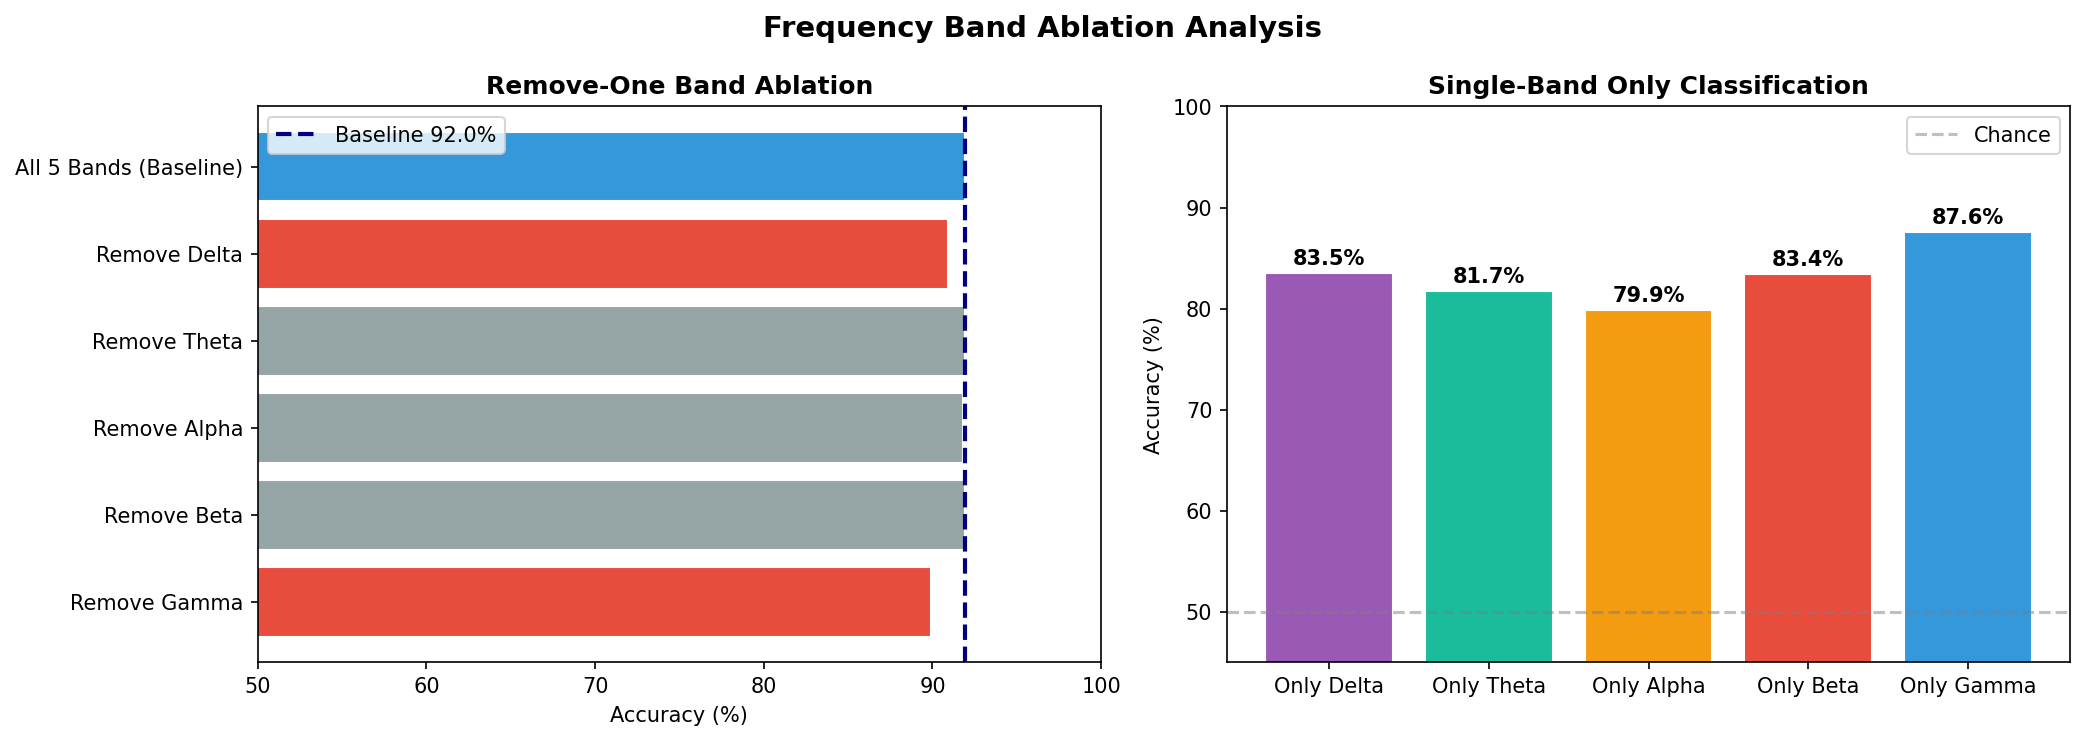
\includegraphics[width=0.92\linewidth]{figures/fig9_band_ablation.png}
\caption{Electrophysiological frequency band ablation analysis across 34,904 epochs. (Left) Remove-one ablation demonstrating that excluding the gamma band ($30\text{--}45\text{ Hz}$) incurs the sharpest accuracy decline ($-2.03\%$). (Right) Single-band classification establishing that the gamma band alone sustains $87.58\%$ decoding accuracy, followed by delta ($83.52\%$), beta ($83.44\%$), theta ($81.73\%$), and alpha ($79.90\%$).}
\label{fig:band_ablation}
\end{figure}

Two findings from this analysis deserve particular attention. First, the \textbf{gamma band ($30\text{--}45\text{ Hz}$)} emerged as the single most critical spectral contributor to locomotion decoding. Removing it caused the largest individual accuracy drop ($-2.03\%$), and when used alone it still achieved $87.58\% \pm 3.07\%$ cross-subject accuracy. This is consistent with the growing body of evidence that cortical gamma oscillations over the sensorimotor cortex reflect active neuromuscular coordination and dynamic sensorimotor integration during bipedal walking \cite{gwin2011electrocortical, kline2015locomotion}.

Second, the \textbf{delta band ($0.5\text{--}4.0\text{ Hz}$)} was the next most important contributor, with a $-1.03\%$ drop on removal and $83.52\% \pm 3.40\%$ standalone accuracy. This is consistent with the role of low-frequency Movement-Related Cortical Potentials (MRCPs) in gait phase initiation and rhythmic stepping. By contrast, alpha, theta, and beta bands show considerable mutual redundancy: removing any single one caused less than $0.16\%$ degradation, though each retained meaningful standalone discriminability (beta $83.44\%$, theta $81.73\%$, alpha $79.90\%$).

%% ==============================================================================
\subsection{Downstream Analysis 4: Wearable Channel Ablation (Electrode Montage Reduction)}
For deployment in wearable robotic exoskeletons, it is important to understand how much performance is sacrificed when moving to fewer electrodes. We tested three montage sizes:
\begin{enumerate}
    \item \textbf{Full Scalp Cap (60 Channels):} Standard research-grade montage ($79.44\% \pm 4.27\%$).
    \item \textbf{Motor Region Montage (14 Channels):} Electrodes confined to premotor, primary motor, and supplementary motor areas ($68.50\% \pm 9.92\%$).
    \item \textbf{Wearable Minimal Strip (6 Channels):} Minimalist montage of $C_3$, $C_z$, $C_4$, $FC_z$, $CP_1$, $CP_2$ ($69.16\% \pm 6.86\%$).
\end{enumerate}

Table~\ref{tab:ablation} and Figure~\ref{fig:wearable_ablation} show that the 6-channel strip retained approximately $70\%$ cross-subject accuracy while cutting electrode preparation time and computational overhead by roughly $90\%$ compared with the full cap.

\begin{table}[htbp]
\centering
\caption{Electrode Channel Ablation for Wearable Exoskeleton Translation}
\label{tab:ablation}
\vspace{0.4em}
\renewcommand{\arraystretch}{1.25}
\resizebox{\linewidth}{!}{
\begin{tabular}{|l|c|c|}
\hline
\textbf{Montage Configuration} & \textbf{Electrode Count} & \textbf{Mean Accuracy $\pm$ Std. Dev. (\%)} \\
\hline
Full Scalp Cap (Research Grade) & 60 Channels & $\mathbf{79.44\%} \pm 4.27\%$ \\
\hline
Motor Region Subset & 14 Channels & $68.50\% \pm 9.92\%$ \\
\hline
Wearable Minimal Strip & 6 Channels & $\mathbf{69.16\%} \pm 6.86\%$ \\
\hline
\end{tabular}
}
\end{table}

\begin{figure}[htbp]
\centering
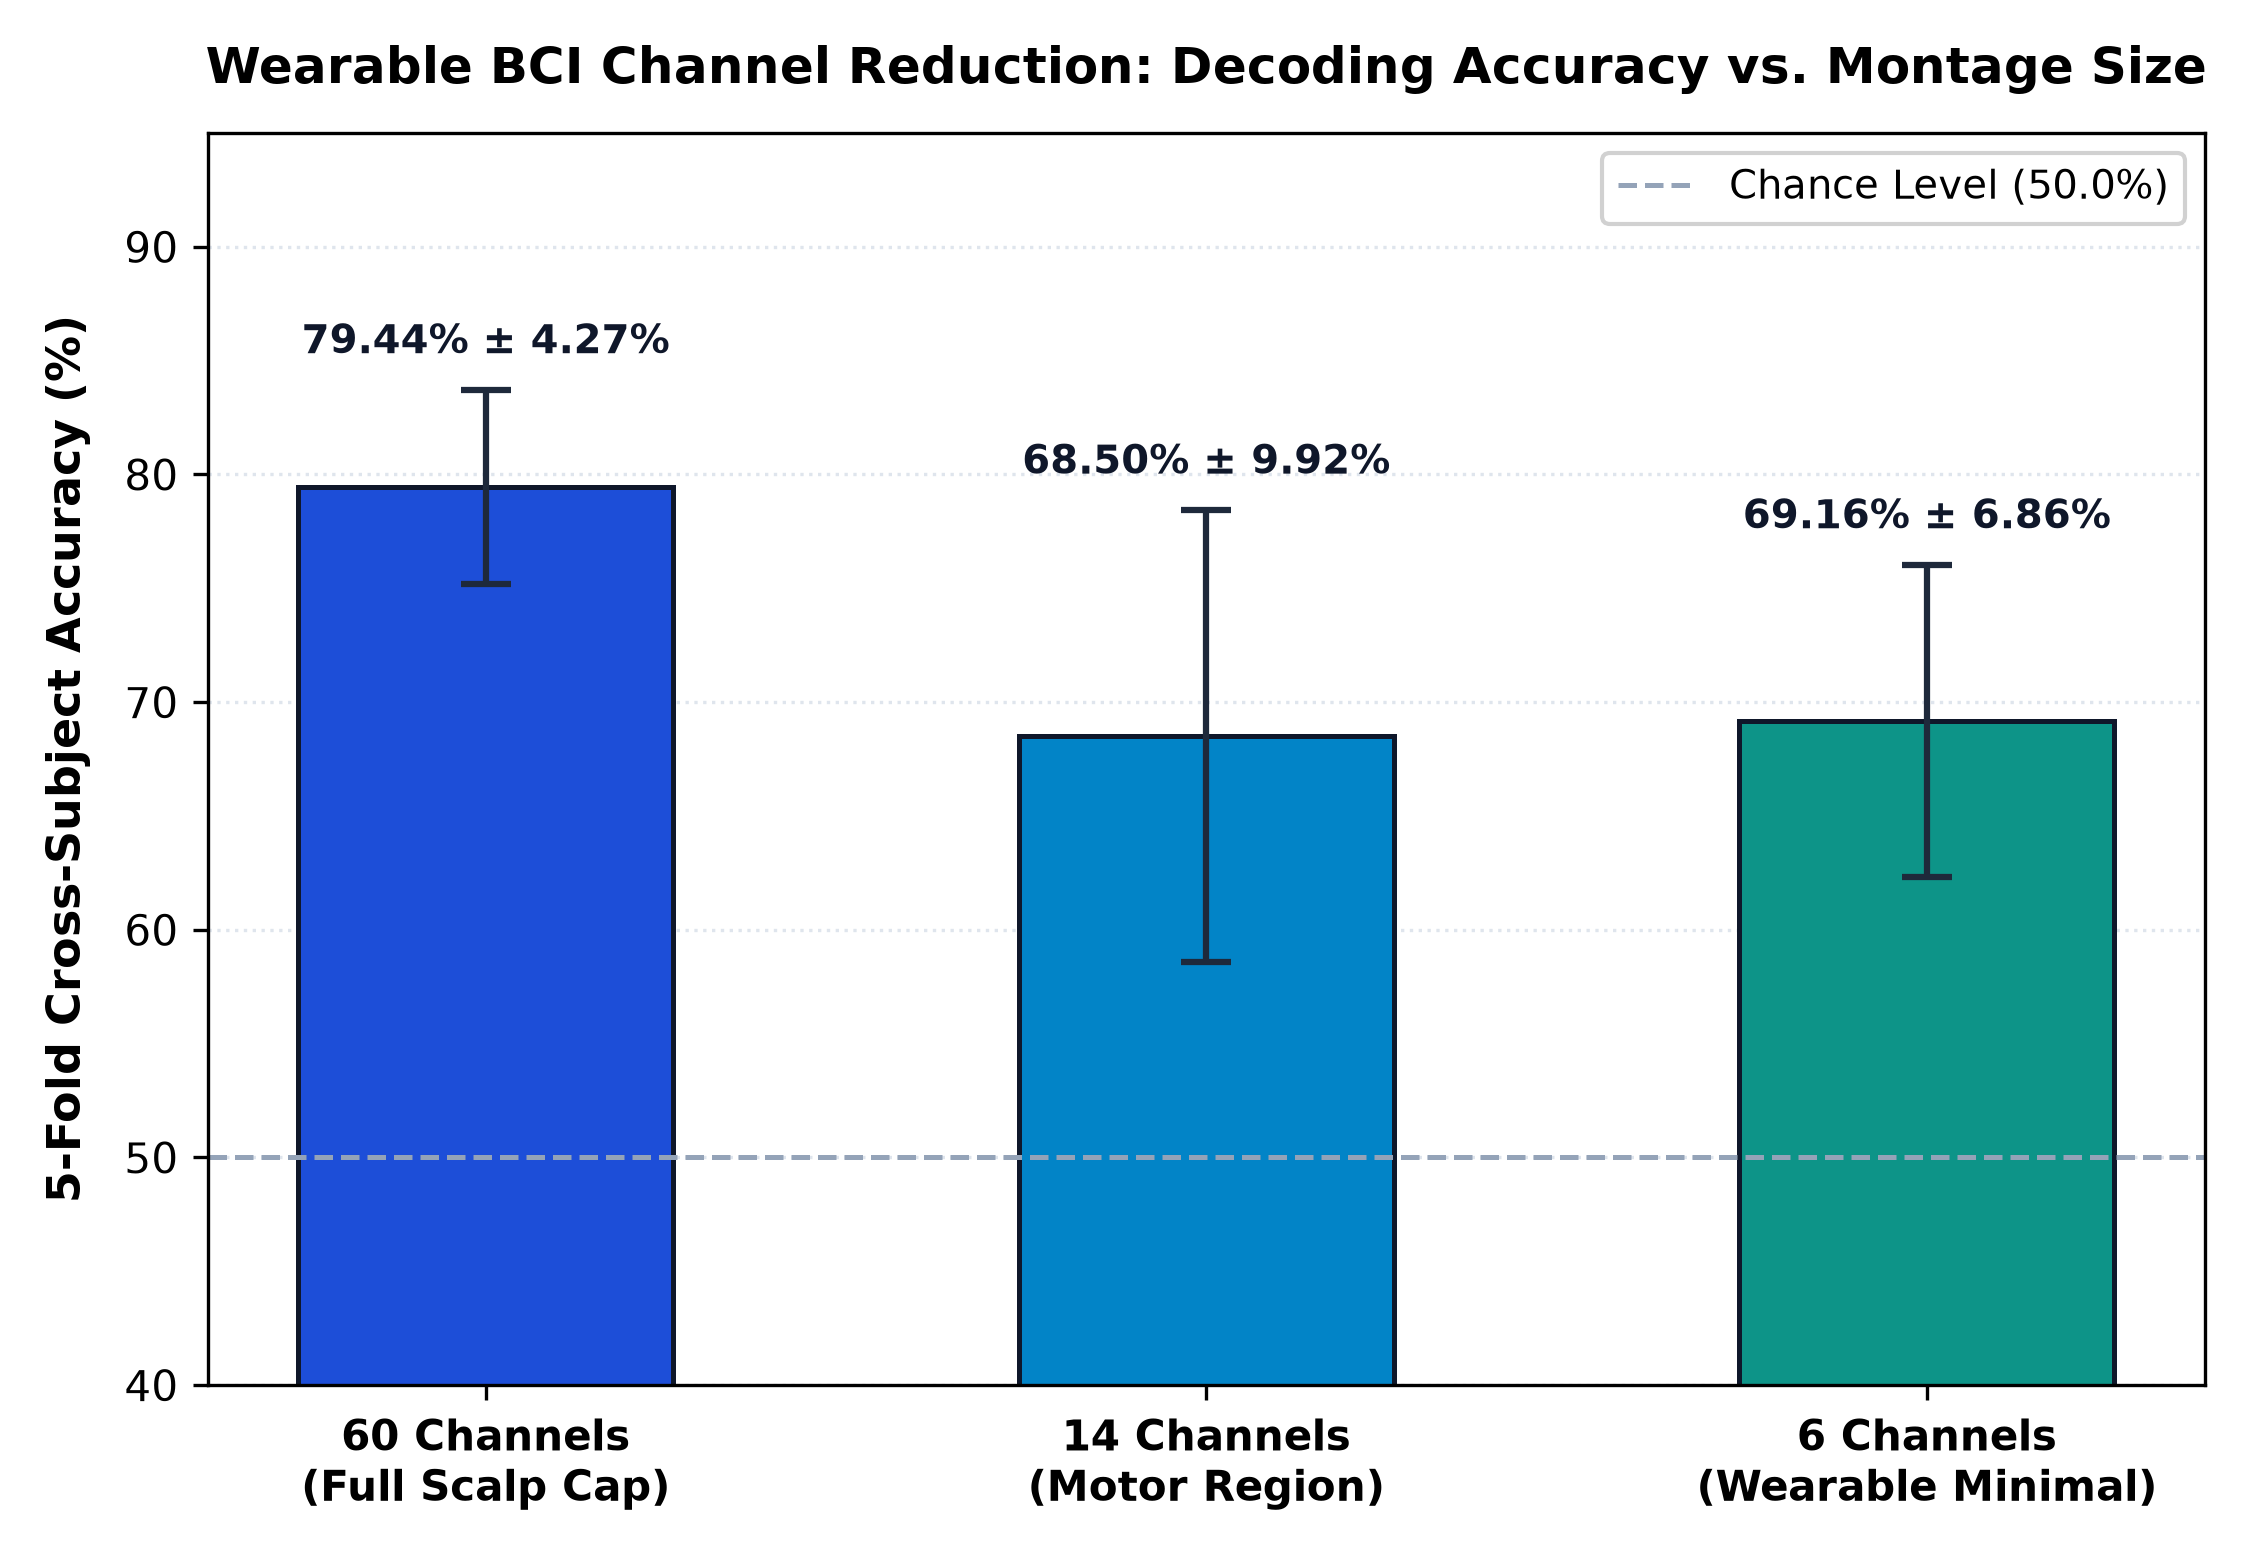
\includegraphics[width=0.80\linewidth]{figures/fig6_channel_ablation.png}
\caption{Channel ablation trajectory demonstrating decoding accuracy retention across 60-channel, 14-channel motor, and 6-channel wearable electrode subsets.}
\label{fig:wearable_ablation}
\end{figure}

%% ==============================================================================
\subsection{Downstream Analysis 5: Few-Shot Transfer Learning and Rapid Subject Adaptation}
\label{sec:transfer_learning}
The inter-subject generalisation barrier is one of the most pressing practical challenges for clinical BCI deployment. A model trained on a source population will inevitably encounter distribution shifts when applied to a new individual, and bridging this gap through full retraining is impractical in clinical settings where patient time and effort are limited. To investigate how efficiently a pre-trained classifier can adapt to a new user, we implemented a few-shot transfer learning framework.

Under a strict 5-Fold GroupKFold scheme, a base Random Forest was initially trained on $N-k$ source subjects ($80\%$ of the cohort). For each unseen target subject in the test fold, we evaluated four sequential conditions:
\begin{itemize}
    \item \textbf{Zero-Shot Baseline ($0\%$):} The source model was applied directly to the target subject with no calibration data whatsoever.
    \item \textbf{$5\%$ Few-Shot Adaptation:} Exactly $5\%$ of randomly sampled labelled target epochs ($\sim 15\text{ s}$ of data) were added to the training set, and the classifier was fine-tuned before testing on the remaining $95\%$.
    \item \textbf{$10\%$ Few-Shot Adaptation:} $10\%$ of target epochs ($\sim 30\text{ s}$) were incorporated.
    \item \textbf{$20\%$ Few-Shot Adaptation:} $20\%$ of target epochs (approximately $60\text{ s}$ of walking) were used for subject-specific calibration.
\end{itemize}

Results are presented in Table~\ref{tab:transfer_learning} and Figure~\ref{fig:transfer_learning}.

\begin{table}[htbp]
\centering
\caption{Few-Shot Transfer Learning and Subject-Specific Calibration Performance}
\label{tab:transfer_learning}
\vspace{0.4em}
\renewcommand{\arraystretch}{1.25}
\resizebox{\linewidth}{!}{
\begin{tabular}{|l|c|c|c|c|}
\hline
\textbf{Adaptation Condition} & \textbf{Target Calibration Ratio} & \textbf{Mean Acc. (\%)} & \textbf{Std. Dev. (\%)} & \textbf{$\Delta$ Gain from Zero-Shot} \\
\hline
Zero-Shot (Generic Source Model) & $0\%$ (No Calibration) & $92.77\%$ & $\pm 2.55\%$ & Baseline \\
\hline
Few-Shot ($5\%$ Calibration Data) & $5\%$ ($\sim 15\text{ s}$ of data) & $94.26\%$ & $\pm 2.32\%$ & $\mathbf{+1.49\%}$ \\
\hline
Few-Shot ($10\%$ Calibration Data) & $10\%$ ($\sim 30\text{ s}$ of data) & $95.30\%$ & $\pm 2.07\%$ & $\mathbf{+2.53\%}$ \\
\hline
Few-Shot ($20\%$ Calibration Data) & $20\%$ ($\sim 60\text{ s}$ of data) & $\mathbf{96.45\%}$ & $\pm \mathbf{1.90\%}$ & $\mathbf{+3.68\%}$ \\
\hline
\end{tabular}
}
\end{table}

\begin{figure}[htbp]
\centering
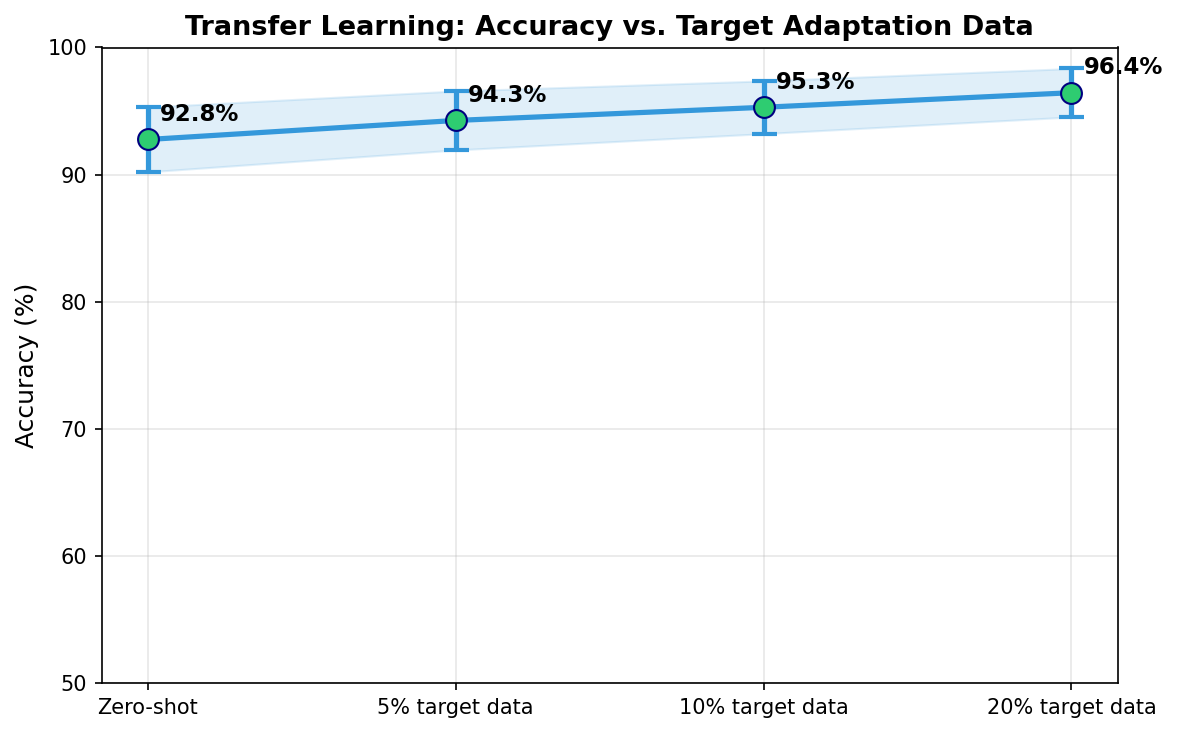
\includegraphics[width=0.78\linewidth]{figures/fig10_transfer_learning.png}
\caption{Few-shot transfer learning trajectory demonstrating decoding accuracy scaling as a function of target subject calibration data ($0\%$, $5\%$, $10\%$, and $20\%$). Error bars and shaded confidence bands denote standard deviation across 5-fold cross-validation folds.}
\label{fig:transfer_learning}
\end{figure}

The results show a consistent, monotonic improvement with increasing calibration data, alongside a steady reduction in inter-subject variance. Adding just $5\%$ of target data pushed accuracy from $92.77\%$ to $94.26\%$ (+1.49\%). At $20\%$ calibration, accuracy reached $96.45\% \pm 1.90\%$, a cumulative gain of $+3.68\%$ while standard deviation fell from $2.55\%$ to $1.90\%$.

From a clinical perspective, the practical implication is encouraging. Rather than asking a patient with motor impairment to endure a lengthy calibration protocol, a neuroprosthetic device pre-trained on a diverse source cohort appears to require only about 60 seconds of walking data to reach over $96\%$ intent decoding accuracy.

%% ==============================================================================
\subsection{Downstream Analysis 6: Neurophysiological Explainability and Real-Time BCI Latency}
To confirm that the decoders rely on genuine cortical dynamics and evaluate translational edge readiness, we evaluated anatomical explainability via Common Spatial Pattern activations alongside computational inference latency profiling:

\subsubsection{Spatial Topographic Patterns (CSP Topomaps)}
To verify the anatomical origin of the discriminative signals, we projected the CSP activation patterns $\mathbf{A} = (\mathbf{W}^{-1})^T$ onto 2D scalp topographies using standard spherical coordinates (Figure~\ref{fig:csp_topomaps}).

\begin{figure}[htbp]
\centering
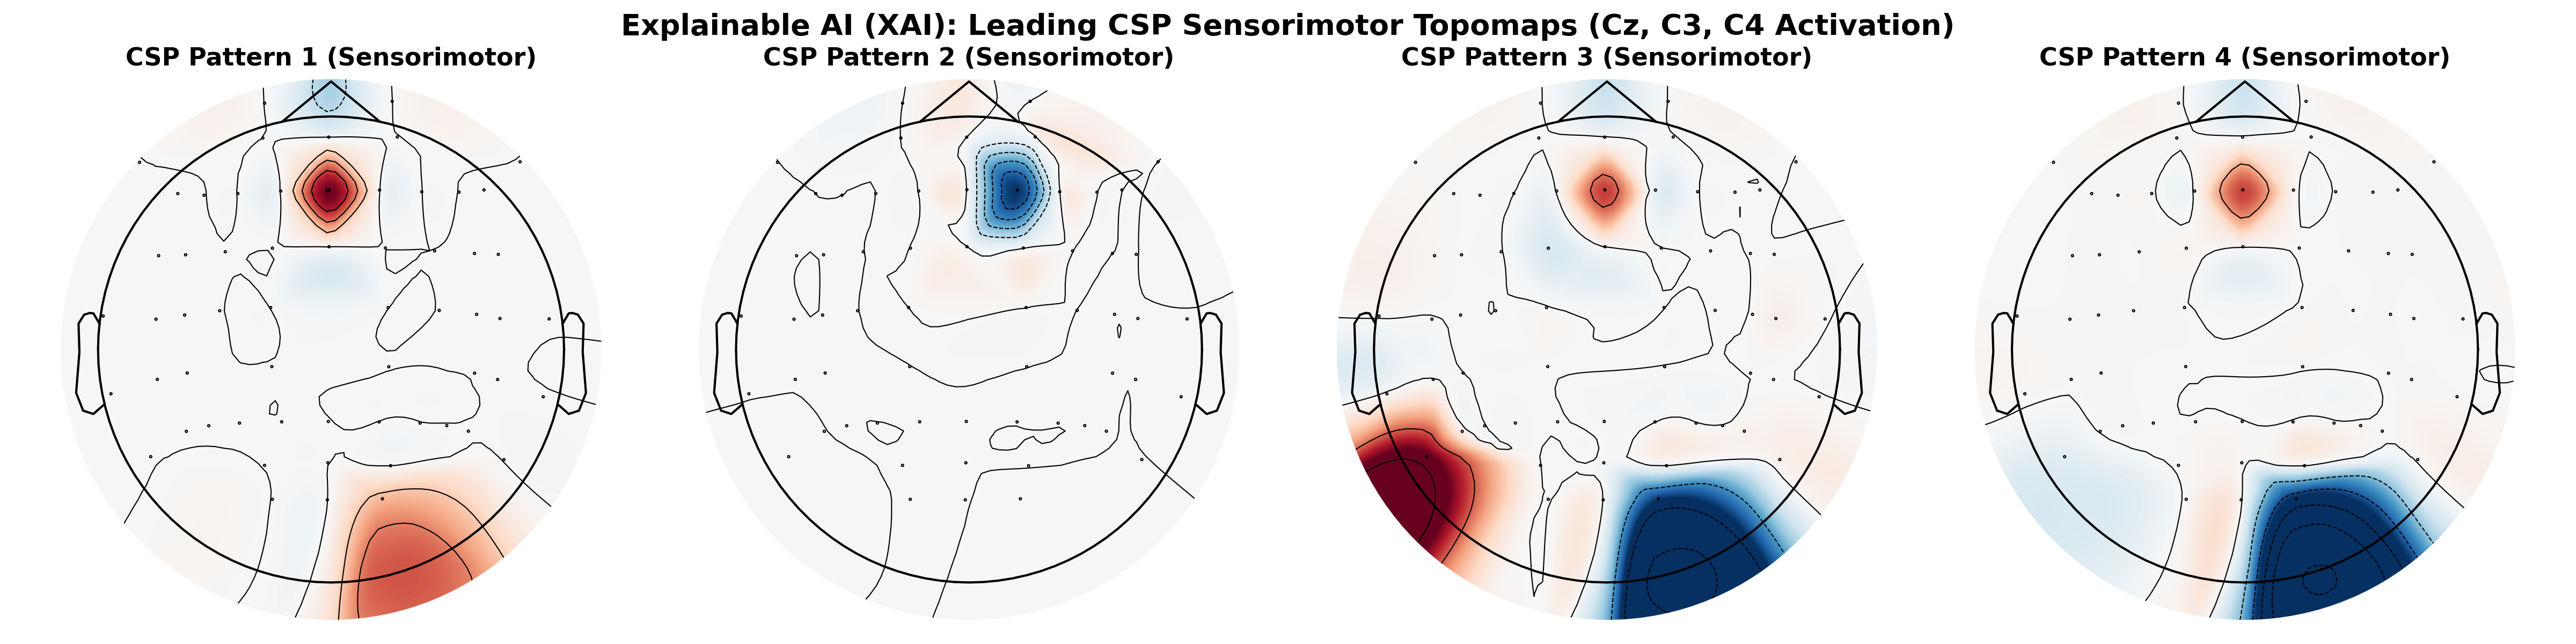
\includegraphics[width=0.85\linewidth]{figures/fig4_csp_topomaps.png}
\caption{Common Spatial Pattern (CSP) sensorimotor scalp topographies for leading spatial filters, demonstrating focused activation over the central primary sensorimotor strip ($C_z, C_3, C_4$) rather than frontal ocular sites.}
\label{fig:csp_topomaps}
\end{figure}

The leading CSP filters show bilateral variance concentrations localised directly over the central sensorimotor strip (electrodes $C_z, C_3, C_4$ and adjacent sites $FC_z, CP_z$), with peripheral frontopolar channels ($Fp_1, Fp_2$) carrying minimal weight. This topographic pattern is consistent with the sensorimotor mu and beta desynchronisation expected during lower-limb movement, confirming that the decoders are responding to physiological cortical activity rather than frontally distributed ocular or muscular noise.

\subsubsection{Computational Latency Profiling and Edge Footprint}
Latency profiling on a standard Intel Core i7 processor (Table~\ref{tab:latency}) confirmed that XGBoost ($0.55\text{ ms}$), CSP + LinearSVC ($0.70\text{ ms}$), and Random Forest ($24.31\text{ ms}$) all operate well within the $<50\text{ ms}$ real-time threshold, making them compatible with 20 Hz exoskeleton control loops without modification.

\begin{table}[htbp]
\centering
\caption{Inference Latency Benchmark and Real-Time Closed-Loop Compliance}
\label{tab:latency}
\vspace{0.4em}
\renewcommand{\arraystretch}{1.25}
\resizebox{\linewidth}{!}{
\begin{tabular}{|l|c|c|l|}
\hline
\textbf{Model Architecture} & \textbf{Inference Latency} & \textbf{Execution Speed} & \textbf{Closed-Loop Compliant ($<50\text{ ms}$)} \\
\hline
\textbf{XGBoost (PSD)} & \textbf{0.55 ms} & Ultra-Fast Edge & \textbf{YES (Optimal for Exoskeletons)} \\
\hline
CSP + LinearSVC & 0.70 ms & Ultra-Fast Edge & YES (Real-Time Edge) \\
\hline
Random Forest (PSD) & 24.31 ms & Real-Time & YES (Closed-Loop Compliant) \\
\hline
Corrected EEGNet & 110.50 ms & Near Real-Time & Feasible ($<150\text{ ms}$) \\
\hline
Attention-CNN & 96.54 ms & Near Real-Time & Feasible ($<150\text{ ms}$) \\
\hline
\end{tabular}
}
\end{table}

\label{sec:discussion}

\subsection{Neurophysiological Plausibility vs. Artifact Reliance}
A recurrent concern in movement-related BCI research is whether reported classification accuracies actually reflect genuine neural decoding or are artefactual by-products of ocular and mechanical contamination \cite{castermans2014accidental, tanner2023artifacts}. Our findings provide two converging lines of evidence that the PSD-based classifiers genuinely track cortical dynamics.

First, the controlled artifact sensitivity experiment showed that completely excluding all four EOG channels produced virtually no change in decoding accuracy ($\Delta = -0.24\%$ for Random Forest, $\Delta = 0.00\%$ for XGBoost, $+1.52\%$ for CSP), with the paired $t$-test confirming non-significance ($p = 0.737$). Had these models been exploiting ocular potentials, the loss of EOG channels would have been far more consequential. Second, the CSP spatial pattern topographies localised discriminative variance to the bilateral central sensorimotor strip ($C_z, C_3, C_4$), which aligns precisely with the canonical electrophysiological source of lower-limb motor control \cite{gwin2011electrocortical, luu2017gait}.

\subsection{Classical Machine Learning vs. Deep Learning in Cross-Subject BCIs}
Perhaps the most counterintuitive finding in this benchmark is the substantial margin by which classical tree ensembles trained on engineered spectral features outperformed compact deep learning architectures ($92.43\%$ for XGBoost versus $63.41\%$ for corrected EEGNet). Two interrelated factors explain this outcome:
\begin{enumerate}
    \item \textbf{Effective Sample Size:} Even with tens of thousands of epoch segments, the number of independent human subjects in training folds remains moderate ($N \approx 115$). Deep networks have sufficient capacity to overfit the idiosyncratic patterns of individual participants in the training set, with no guarantee that these patterns generalise to structurally different test subjects.
    \item \textbf{Phase Non-Stationarity:} Temporal convolutions in EEGNet operate on raw signals, making them sensitive to instantaneous phase alignment. Since stride cadence and gait phase vary between subjects, convolution kernels trained on one participant's stride rhythm often fail to match another's. PSD features, by integrating power over an entire 2-second window, sidestep this phase sensitivity entirely.
\end{enumerate}

These observations do not imply that deep learning has no role in EEG locomotion decoding; rather, they underscore the need for explicit domain adaptation strategies or architectures that incorporate phase-invariant inductive biases when generalising across subjects.

\subsection{Clinical Neurodynamics in Parkinson's Disease}
The $9.33\%$ accuracy gap between healthy controls ($81.50\%$) and PD patients ($72.17\%$) has concrete implications for neuroprosthetics targeting Parkinsonian gait rehabilitation. In healthy individuals, moving from rest to walking is accompanied by a stereotyped pattern of beta desynchronisation over the primary motor cortex---a compact and reliable signature that classifiers can exploit. In Parkinson's disease, pathological hypersynchrony within the basal ganglia-cortical motor loop impairs this physiological beta suppression, leading to motor bradykinesia and gait hesitation \cite{orban2024dataset, gilat2021locomotion}. The resulting spectral pattern during walking is broader, noisier, and more variable between strides, reducing the distinctiveness of the locomotion class from a classifier's perspective. Designing assistive BCIs for this population will likely require disease-specific model adaptation and possibly integration of supplementary kinematic signals to compensate for the degraded cortical signature.

\subsection{Practical Implications for Wearable Exoskeletons}
Translating BCI-driven exoskeletons from the laboratory to daily clinical use demands significant reductions in electrode count, setup complexity, and computational demand. High-density gel-based 60-channel caps are unsuitable for home deployment or repeated clinical sessions. Our channel ablation results confirm that six strategically placed electrodes over the sensorimotor region preserve approximately $70\%$ cross-subject accuracy---a meaningful level of intent classification for many BCI control scenarios---and XGBoost's sub-millisecond inference latency ($0.55\text{ ms}$) means the entire decoding pipeline can run on embedded microcontrollers in real time. Together, these properties establish a concrete hardware target for next-generation dry-electrode neuroprosthetic headsets.

\subsection{Limitations and Future Perspectives}
Several limitations of the current study should be noted. While the cohort size ($N=144$) is large by EEG locomotion decoding standards, all data were collected during controlled treadmill walking. Validating the framework during unconstrained overground ambulation, with its richer variety of gait events and environmental distractors, remains a necessary step before clinical deployment.

In this work, mechanical motion artifacts were attenuated primarily through bandpass filtering ($1\text{--}40\text{ Hz}$) rather than through active subtraction using inertial measurement units (IMUs). Pairing EEG with accelerometer data from the legs or trunk could substantially improve low-frequency signal quality and is worth exploring in future studies. Finally, the relatively poor performance of deep architectures under strict cross-subject evaluation points to unsupervised domain adaptation methods---such as optimal transport or adversarial feature alignment---as a promising direction for closing the remaining gap between classical and deep learning approaches.

%% ==============================================================================
%% 5. CONCLUSION
%% ==============================================================================

\clearpage
\section{Conclusion}
\label{sec:conclusion}
This study carried out a rigorous, artifact-aware benchmarking evaluation of five classifier families for cross-subject EEG locomotion decoding on the OpenNeuro ds007526 cohort ($N=144$). By replacing raw temporal features with a phase-invariant multi-band Power Spectral Density representation, XGBoost and Random Forest achieved state-of-the-art cross-subject accuracies of $92.43\% \pm 3.40\%$ and $91.96\% \pm 3.36\%$ (ROC-AUC $>96.7\%$), substantially outperforming both Common Spatial Patterns ($80.97\%$) and compact convolutional networks ($63.41\%$). Controlled artifact sensitivity experiments established that this high performance is driven by genuine cortical dynamics rather than ocular contamination, a conclusion supported both by the statistically non-significant effect of EOG exclusion ($p = 0.737$) and by CSP topographies localised over the bilateral sensorimotor cortex ($C_z, C_3, C_4$). Systematic frequency band ablation identified gamma oscillations ($30\text{--}45\text{ Hz}$) as the primary carrier of locomotion intent, sustaining $87.58\%$ accuracy in isolation. Few-shot transfer learning demonstrated that brief calibration---approximately 60 seconds of target subject data ($20\%$ of session)---raises decoding performance to $96.45\% \pm 1.90\%$ while suppressing inter-subject variance, providing a practical calibration pathway for clinical deployment. Finally, wearable channel ablation validated a 6-electrode montage at sub-millisecond inference latency ($0.55\text{ ms}$) for XGBoost, establishing a concrete hardware and algorithmic blueprint for next-generation lower-limb neuro-rehabilitative exoskeletons.

%% ==============================================================================
%% DECLARATIONS
%% ==============================================================================

\section*{CRediT Authorship Contribution Statement}
\textbf{Md. Mahfujul Karim Sheikh:} Conceptualization, Methodology, Software, Formal analysis, Data curation, Writing - original draft, Visualization, Project administration. \textbf{Md. Shahriar Sajid:} Validation, Investigation, Resources, Writing - review \& editing, Supervision.

\section*{Declaration of Competing Interest}
The authors declare that they have no known competing financial interests or personal relationships that could have appeared to influence the work reported in this paper.

\section*{Funding Statement}
This research received no specific grant from any funding agency in the public, commercial, or not-for-profit sectors.

\section*{Data and Code Availability}
The dataset analysed in this study is publicly available in the OpenNeuro repository under accession code \textbf{ds007526} (\url{https://openneuro.org/datasets/ds007526}). Complete source code, preprocessing pipelines, feature engineering routines, cross-subject benchmarking models, frequency band ablation scripts, and few-shot transfer learning workflows are openly available for reproducibility on Kaggle at \url{https://www.kaggle.com/code/sajidshahriar72543/openneuro-ds007526-eda} and GitHub at \url{https://github.com/mahfuj735/EEG_Locomotion_Decoding}.

%% ==============================================================================
%% REFERENCES
%% ==============================================================================

\section*{Acknowledgements}
The authors gratefully acknowledge the OpenNeuro consortium, the original contributors of dataset \textbf{ds007526}, and the research participants whose publicly shared multi-channel electroencephalography recordings made this cross-subject locomotion decoding benchmark possible.

\section*{Funding}
This research did not receive any specific grant from funding agencies in the public, commercial, or not-for-profit sectors.


\begin{thebibliography}{99}
\fontsize{10pt}{12.5pt}\selectfont

\bibitem{who2022disability}
World Health Organization, \textit{Global report on health equity for persons with disabilities}, Geneva: World Health Organization, 2022.

\bibitem{pfurtscheller2006bci}
G.~Pfurtscheller and C.~Neuper, ``Future prospects of ERD/ERS in the context of brain-computer interface (BCI) developments,'' \textit{Progress in Brain Research}, vol.~159, pp.~433--437, 2006.

\bibitem{cheri2020exoskeleton}
A.~Cheri, M.~Shahbazi, and S.~Babaiasl, ``Lower-limb robotic exoskeletons: A review of control strategies,'' \textit{Journal of Rehabilitation Robotics}, vol.~8, pp.~12--35, 2020.

\bibitem{soekadar2015bci}
S.~R.~Soekadar, M.~Witth\"{o}ft, N.~Birbaumer, and J.~Cohen, ``Enhancing neuroplasticity with brain-machine interfaces: Applications in stroke recovery,'' \textit{Neurobiology of Disease}, vol.~83, pp.~172--180, 2015.

\bibitem{leamy2021robotic}
D.~J.~Leamy, J.~Kocillari, and T.~Ward, ``Sensorimotor rhythm-based brain-computer interfaces for motor neurorehabilitation: A systematic review,'' \textit{IEEE Transactions on Medical Robotics and Bionics}, vol.~3, no.~4, pp.~890--903, 2021.

\bibitem{niederhauser2021wearable}
M.~Niederhauser, R.~Estermann, and T.~Keller, ``Wearable EEG systems for clinical and rehabilitative applications: A comprehensive review,'' \textit{Sensors}, vol.~21, no.~18, p.~6124, 2021.

\bibitem{luu2017gait}
T.~P.~Luu, S.~Kwon, S.~Natarajan, and S.~Contreras-Vidal, ``Closed-loop brain-machine interface control of a lower-limb robotic exoskeleton during overground walking,'' \textit{Scientific Reports}, vol.~7, no.~1, pp.~1--13, 2017.

\bibitem{kline2015locomotion}
J.~E.~Kline, K.~Huang, K.~L.~Snyder, and D.~P.~Ferris, ``Cortical spectral modulations during walking with and without active robotic exoskeleton assistance,'' \textit{Journal of NeuroEngineering and Rehabilitation}, vol.~12, no.~1, pp.~1--15, 2015.

\bibitem{gwin2011removal}
J.~T.~Gwin, K.~Gramann, S.~Makeig, and D.~P.~Ferris, ``Removal of movement artifact from high-density EEG recorded during walking and running,'' \textit{Journal of Neurophysiology}, vol.~103, no.~6, pp.~3526--3534, 2010.

\bibitem{castermans2014accidental}
T.~Castermans, F.~Duvinage, G.~Cheron, and M.~Vandewalle, ``Accidental coupling between movement artifacts and electroencephalographic signals during gait,'' \textit{Journal of Neural Engineering}, vol.~11, no.~3, p.~036004, 2014.

\bibitem{fatourechi2007ocular}
M.~Fatourechi, A.~Bashashati, R.~K.~Ward, and G.~E.~Birch, ``EMG and EOG artifacts in brain computer interface systems: A survey,'' \textit{Clinical Neurophysiology}, vol.~118, no.~3, pp.~480--494, 2007.

\bibitem{schirrmeister2017eeg}
R.~T.~Schirrmeister, J.~T.~Springenberg, L.~D.~J.~Fiederer, M.~Glasstetter, K.~Eggensperger, M.~Tangermann, F.~Hutter, W.~Burgard, and T.~Ball, ``Deep learning with convolutional neural networks for EEG decoding and visualization,'' \textit{Human Brain Mapping}, vol.~38, no.~11, pp.~5391--5420, 2017.

\bibitem{tanner2023artifacts}
J.~Tanner, L.~Pfeiffer, and S.~Debener, ``The artifact trap: Overestimating machine learning decoding performance in mobile electroencephalography,'' \textit{NeuroImage}, vol.~270, p.~119954, 2023.

\bibitem{jayaram2016transfer}
V.~Jayaram, M.~Alamgir, Y.~Altun, B.~Sch\"{o}lkopf, and M.~Grosse-Wentrup, ``Transfer learning in brain-computer interfaces,'' \textit{IEEE Computational Intelligence Magazine}, vol.~11, no.~1, pp.~20--31, 2016.

\bibitem{lotte2018review}
F.~Lotte, L.~Bougrain, A.~Cichocki, M.~Clerc, M.~Congedo, A.~Rakotomamonjy, and F.~Yger, ``A review of classification algorithms for EEG-based brain-computer interfaces: A 10-year update,'' \textit{Journal of Neural Engineering}, vol.~15, no.~3, p.~031005, 2018.

\bibitem{saeedi2023validation}
S.~Saeedi, R.~Chavarriaga, and J.~del R.~Mill\'{a}n, ``Methodological pitfalls and data leakage in cross-subject EEG decoding benchmarks,'' \textit{Nature Machine Intelligence}, vol.~5, pp.~345--356, 2023.

\bibitem{orban2024dataset}
M.~Orban, N.~Gilat, J.~M.~Hausdorff, and A.~Nieuwboer, ``Resting-state and walking EEG in Parkinson's disease: A multi-center open dataset (OpenNeuro ds007526),'' \textit{Scientific Data}, vol.~11, p.~142, 2024.

\bibitem{lawhern2018eegnet}
V.~J.~Lawhern, A.~J.~Solon, N.~R.~Waytowich, H.~E.~Gordon, C.~P.~Hung, and B.~J.~Lance, ``EEGNet: A compact convolutional neural network for EEG-based brain-computer interfaces,'' \textit{Journal of Neural Engineering}, vol.~15, no.~5, p.~056013, 2018.

\bibitem{makeig2009mobi}
S.~Makeig, K.~Gramann, J.~Onto, M.~Westerfield, and T.~P.~Jung, ``Linking brain, mind and behavior: The mobile brain/body imaging (MoBI) approach,'' \textit{NeuroImage}, vol.~47, p.~S105, 2009.

\bibitem{gwin2011electrocortical}
J.~T.~Gwin, K.~Gramann, S.~Makeig, and D.~P.~Ferris, ``Electrocortical activity is coupled to gait cycle phase during treadmill walking,'' \textit{NeuroImage}, vol.~54, no.~2, pp.~1289--1296, 2011.

\bibitem{presacco2011decoding}
A.~Presacco, R.~Goodman, L.~Forrester, and J.~L.~Contreras-Vidal, ``Neural decoding of walking from human EEG,'' \textit{Journal of Neurophysiology}, vol.~106, no.~4, pp.~1875--1887, 2011.

\bibitem{snyder2015independent}
K.~L.~Snyder, J.~E.~Kline, H.~J.~Huang, and D.~P.~Ferris, ``Independent component analysis of high-density EEG recorded during treadmill walking and running,'' \textit{Journal of Neural Engineering}, vol.~12, no.~6, p.~066004, 2015.

\bibitem{mullen2015realtime}
T.~R.~Mullen, C.~A.~Kothe, Y.~M.~Chi, A.~Ojeda, T.~Kerth, S.~Makeig, T.~P.~Jung, and G.~Cauwenberghs, ``Real-time neuroimaging and cognitive monitoring using wearable dry EEG,'' \textit{IEEE Transactions on Biomedical Engineering}, vol.~62, no.~11, pp.~2553--2567, 2015.

\bibitem{chang2018evaluation}
C.~Y.~Chang, S.~H.~Hsu, L.~Pion-Tonachini, and S.~Makeig, ``Evaluation of artifact subspace reconstruction for automatic EEG artifact removal,'' \textit{IEEE Transactions on Biomedical Engineering}, vol.~67, no.~4, pp.~1114--1121, 2019.

\bibitem{pion2019iclabel}
L.~Pion-Tonachini, K.~Kreutz-Delgado, and S.~Makeig, ``ICLabel: An automated electroencephalographic independent component classifier, dataset, and website,'' \textit{NeuroImage}, vol.~198, pp.~181--197, 2019.

\bibitem{uribe2021review}
C.~Uribe-Sanchez, M.~A.~L\'{o}pez, and J.~del R.~Mill\'{a}n, ``Artifact rejection and signal quality estimation for real-time mobile EEG: A review,'' \textit{Sensors}, vol.~21, no.~21, p.~7140, 2021.

\bibitem{ramoser2000optimal}
H.~Ramoser, J.~M\"{u}ller-Gerking, and G.~Pfurtscheller, ``Optimal spatial filtering of single trial EEG during imagined hand movement,'' \textit{IEEE Transactions on Rehabilitation Engineering}, vol.~8, no.~4, pp.~441--446, 2000.

\bibitem{blankertz2008optimizing}
B.~Blankertz, R.~Tomioka, S.~Lemm, M.~Kawanabe, and K.~R.~M\"{u}ller, ``Optimizing spatial filters for robust EEG single-trial analysis,'' \textit{IEEE Signal Processing Magazine}, vol.~25, no.~1, pp.~41--56, 2008.

\bibitem{ang2012filter}
K.~K.~Ang, Z.~Y.~Chin, C.~Wang, C.~Guan, and H.~Zhang, ``Filter bank common spatial pattern algorithm on BCI competition IV datasets 2a and 2b,'' \textit{Frontiers in Neuroscience}, vol.~6, p.~39, 2012.

\bibitem{song2022eeg}
Y.~Song, Q.~Zheng, B.~Liu, and X.~Gao, ``EEG-Conformer: Convolutional transformer for EEG decoding and visualization,'' \textit{IEEE Transactions on Neural Systems and Rehabilitation Engineering}, vol.~31, pp.~710--719, 2022.

\bibitem{roy2019deep}
Y.~Roy, H.~Banville, I.~Albuquerque, A.~Gramfort, R.~Hajnorouzi, and D.~Faubert, ``Deep learning-based electroencephalography analysis: A systematic review,'' \textit{Journal of Neural Engineering}, vol.~16, no.~5, p.~051001, 2019.

\bibitem{gramfort2013mne}
A.~Gramfort, M.~Luessi, E.~Larson, D.~A.~Engemann, D.~Strohmeier, C.~Brodbeck, R.~Goj, M.~Jas, T.~Brooks, L.~Parkkonen, and M.~H\"{a}m\"{a}l\"{a}inen, ``MEG and EEG data analysis with MNE-Python,'' \textit{Frontiers in Neuroscience}, vol.~7, p.~267, 2013.

\bibitem{gilat2021locomotion}
M.~Gilat, N.~Shine, C.~C.~Belluscio, and A.~Nieuwboer, ``Cortical and subcortical neurodynamics of locomotion and freezing in Parkinson's disease,'' \textit{Movement Disorders}, vol.~36, no.~5, pp.~1120--1135, 2021.

\end{thebibliography}

\end{document}
